\documentclass[10pt]{article}


% macros.tex
\usepackage{amsmath}
\usepackage{amsfonts}
\usepackage{amssymb}
\usepackage{amsthm}


% You change everything, by adding \usepackage{times} to the document
% Preamble. Now all the roman letters will be set in times and all the
% sans serif stuff will be set in Helvetica. If you don't like times,
% you can try the packages: palatcm, charter, helvet, palatino, avant,
% newcent and bookman
% If you want to change explicitly to a certain font, use the command
% \fontfamily{XYZ}\selectfont whereby XYZ can be set to: pag for Adobe
% AvantGarde, pbk for Adobe Bookman, pcr for Adobe Courier, phv for
% Adobe Helvetica, pnc for Adobe NewCenturySchoolbook, ppl for Adobe
% Palatino, ptm for Adobe Times Roman, pzc for Adobe ZapfChancery
\newcommand{\courier}{\fontfamily{pcr}\selectfont}



\newcommand{\edit}[1]{\footnote{[[#1]]}\marginpar{\hfill {\sf[[\thefootnote]]}}}
%\newcommand{\edit}[1]{{\sl\small [[Todo: #1]]}}


%\author{William~A. Stein}

\newcommand{\Hbar}{\overline{H}}

\newcommand{\myhead}[3]{
\par\noindent
{Version #2}
\vspace{10ex}
\par\noindent
{\bf \LARGE #1}\\
\vspace{3ex}
\par\noindent
{\large W.\thinspace{}A. Stein}\\
{\small Department of Mathematics, Harvard University}\vspace{1ex}\\
#3     
\vspace{2ex}\par
}

\newcommand{\myheadauth}[3]{
\par\noindent
{Version #2}
\vspace{10ex}
\par\noindent
{\bf \LARGE #1}\\
\vspace{3ex}
\par\noindent
#3     
\vspace{5ex}\par
}

\usepackage{xspace}  % to allow for text macros that don't eat space 
\newcommand{\SAGE}{{\sf Sage}\xspace}
\newcommand{\sage}{\SAGE}
\newcommand{\gzero}{\Gamma_0(N)}
\newcommand{\esM}{\overline{\sM}}
\newcommand{\sM}{\boldsymbol{\mathcal{M}}}
\newcommand{\sS}{\boldsymbol{\mathcal{S}}}
\newcommand{\sB}{\boldsymbol{\mathcal{B}}}       
\newcommand{\eE}{\mathbb{E}}
\newcommand{\bA}{\mathbb{A}}
\newcommand{\cK}{\mathcal{K}}
\newcommand{\Adual}{A^{\vee}}
\newcommand{\Bdual}{B^{\vee}}

\newcommand{\defn}[1]{{\em #1}}
\newcommand{\solution}[1]{\vspace{1em}%
  \par\noindent{\bf Solution #1.} }
\newcommand{\todo}[1]{\noindent$\bullet$ {\small \textsf{#1}} $\bullet$\\}
\newcommand{\done}[1]{\noindent {\small \textsf{Done: #1}}\\}
\newcommand{\danger}[1]{\marginpar{\small \textsl{#1}}}
\renewcommand{\div}{\mbox{\rm div}}
\DeclareMathOperator{\GCD}{GCD}
\DeclareMathOperator{\sss}{ss}
\renewcommand{\ss}{\sss}
\DeclareMathOperator{\red}{red}
\DeclareMathOperator{\sat}{sat}
\DeclareMathOperator{\xgcd}{xgcd}
\DeclareMathOperator{\Kol}{Kol}
\DeclareMathOperator{\can}{can}
\DeclareMathOperator{\Cl}{Cl}
\DeclareMathOperator{\Mod}{Mod}
\DeclareMathOperator{\chr}{char}
\DeclareMathOperator{\charpoly}{charpoly}
\DeclareMathOperator{\cris}{cris}
\DeclareMathOperator{\dR}{dR}
\DeclareMathOperator{\Fil}{Fil}
\DeclareMathOperator{\ind}{ind}
\DeclareMathOperator{\im}{im}
\DeclareMathOperator{\oo}{\infty}
\DeclareMathOperator{\abs}{abs}
\DeclareMathOperator{\lcm}{lcm}
\DeclareMathOperator{\cores}{cores}
\DeclareMathOperator{\coker}{coker}
\DeclareMathOperator{\image}{image}
\DeclareMathOperator{\prt}{part}
\DeclareMathOperator{\proj}{proj}
\DeclareMathOperator{\Br}{Br}
\DeclareMathOperator{\Ann}{Ann}
\DeclareMathOperator{\End}{End}
\DeclareMathOperator{\Tan}{Tan}
\DeclareMathOperator{\Eis}{Eis}
\newcommand{\unity}{\mathbb{1}}
\DeclareMathOperator{\Pic}{Pic}
\DeclareMathOperator{\Tate}{Tate}
\DeclareMathOperator{\Vol}{Vol}
\DeclareMathOperator{\Vis}{Vis}
\DeclareMathOperator{\Reg}{Reg}
%\DeclareMathOperator{\myRes}{Res}
%\newcommand{\Res}{\myRes}
\DeclareMathOperator{\Res}{Res}
\newcommand{\an}{{\rm an}}
\DeclareMathOperator{\rank}{rank}
\DeclareMathOperator{\Sel}{Sel}
\DeclareMathOperator{\Mat}{Mat}
\DeclareMathOperator{\BSD}{BSD}
\DeclareMathOperator{\id}{id}
\DeclareMathOperator{\dz}{dz}
%\DeclareMathOperator{\Re}{Re}
\renewcommand{\Re}{\mbox{\rm Re}}
\DeclareMathOperator{\Imm}{Im}
\renewcommand{\Im}{\Imm}
\DeclareMathOperator{\Selmer}{Selmer}
\newcommand{\pfSel}{\widehat{\Sel}}
\newcommand{\qe}{\stackrel{\mbox{\tiny ?}}{=}}
\newcommand{\isog}{\simeq}
\newcommand{\e}{\mathbf{e}}
\newcommand{\bN}{\mathbf{N}}

% ---- SHA ----
\DeclareFontEncoding{OT2}{}{} % to enable usage of cyrillic fonts
  \newcommand{\textcyr}[1]{%
    {\fontencoding{OT2}\fontfamily{wncyr}\fontseries{m}\fontshape{n}%
     \selectfont #1}}
\newcommand{\Sha}{{\mbox{\textcyr{Sh}}}}

%\font\cyr=wncyr10 scaled \magstep 1
%\font\cyr=wncyr10

%\newcommand{\Sha}{{\cyr X}}
\newcommand{\Shaan}{\Sha_{\mbox{\tiny \rm an}}}
\newcommand{\TS}{Shafarevich-Tate group}

\newcommand{\Gam}{\Gamma}
\newcommand{\X}{\mathcal{X}}
\newcommand{\cH}{\mathcal{H}}
\newcommand{\cA}{\mathcal{A}}
\newcommand{\cF}{\mathcal{F}}
\newcommand{\cG}{\mathcal{G}}
\newcommand{\cJ}{\mathcal{J}}
\newcommand{\cL}{\mathcal{L}}
\newcommand{\cV}{\mathcal{V}}
\newcommand{\cO}{\mathcal{O}}
\newcommand{\cQ}{\mathcal{Q}}
\newcommand{\cX}{\mathcal{X}}
\newcommand{\ds}{\displaystyle}
\newcommand{\M}{\mathcal{M}}
\newcommand{\E}{\mathcal{E}}
\renewcommand{\L}{\mathcal{L}}
\newcommand{\J}{\mathcal{J}}
\DeclareMathOperator{\new}{new}
\DeclareMathOperator{\Morph}{Morph}
\DeclareMathOperator{\old}{old}
\DeclareMathOperator{\Sym}{Sym}
\DeclareMathOperator{\Symb}{Symb}
%\newcommand{\Sym}{\mathcal{S}{\rm ym}}
\newcommand{\dw}{\delta(w)} 
\newcommand{\dwh}{\widehat{\delta(w)}}      
\newcommand{\dlwh}{\widehat{\delta_\l(w)}} 
\newcommand{\dash}{-\!\!\!\!-\!\!\!\!-\!\!\!\!-} 
\DeclareMathOperator{\tor}{tor}  
\newcommand{\Frobl}{\Frob_{\ell}}
\newcommand{\tE}{\tilde{E}}
\renewcommand{\l}{\ell}
\renewcommand{\t}{\tau}
\DeclareMathOperator{\cond}{cond}
\DeclareMathOperator{\Spec}{Spec}
\DeclareMathOperator{\Div}{Div}
\DeclareMathOperator{\Jac}{Jac}
\DeclareMathOperator{\res}{res}
\DeclareMathOperator{\Ker}{Ker}
\DeclareMathOperator{\Coker}{Coker}
\DeclareMathOperator{\sep}{sep}
\DeclareMathOperator{\sign}{sign}
\DeclareMathOperator{\unr}{unr}
\newcommand{\N}{\mathcal{N}}
\newcommand{\U}{\mathcal{U}}
\newcommand{\Kbar}{\overline{K}}
\newcommand{\Lbar}{\overline{L}}
\newcommand{\gammabar}{\overline{\gamma}}
\newcommand{\q}{\mathbf{q}}
%\renewcommand{\star}{\times}
\newcommand{\gM}{\mathfrak{M}}
\newcommand{\gA}{\mathfrak{A}}
\newcommand{\gP}{\mathfrak{P}}
\newcommand{\bmu}{\boldsymbol{\mu}}
\newcommand{\union}{\cup}
\newcommand{\Tl}{T_{\ell}}
\newcommand{\into}{\rightarrow}
\newcommand{\onto}{\rightarrow\!\!\!\!\rightarrow}
\newcommand{\intersect}{\cap}
\newcommand{\meet}{\cap}
\newcommand{\cross}{\times}
\DeclareMathOperator{\md}{mod}
\DeclareMathOperator{\toric}{toric}
\DeclareMathOperator{\tors}{tors}
\DeclareMathOperator{\Frac}{Frac}
\DeclareMathOperator{\corank}{corank}
\newcommand{\kr}[2]{\left(\frac{#1}{#2}\right)}
\newcommand{\rb}{\overline{\rho}}
\newcommand{\ra}{\rightarrow}
\newcommand{\xra}[1]{\xrightarrow{#1}}
\newcommand{\hra}{\hookrightarrow}
\newcommand{\la}{\leftarrow}
\newcommand{\lra}{\longrightarrow}
\newcommand{\riso}{\xrightarrow{\sim}}
\newcommand{\da}{\downarrow}
\newcommand{\ua}{\uparrow}
\newcommand{\con}{\equiv}
\newcommand{\Gm}{\mathbb{G}_m}
\newcommand{\pni}{\par\noindent}
\newcommand{\set}[1]{\left\{#1\right\}}
\newcommand{\iv}{^{-1}}
\newcommand{\alp}{\alpha}
\newcommand{\bq}{\mathbf{q}}
\newcommand{\cpp}{{\tt C++}}
\newcommand{\tensor}{\otimes}
\newcommand{\bg}{{\tt BruceGenus}}
\newcommand{\abcd}[4]{\left(
        \begin{smallmatrix}#1&#2\\#3&#4\end{smallmatrix}\right)}
\newcommand{\mthree}[9]{\left(
        \begin{matrix}#1&#2&#3\\#4&#5&#6\\#7&#8&#9
        \end{matrix}\right)}
\newcommand{\mtwo}[4]{\left(
        \begin{matrix}#1&#2\\#3&#4
        \end{matrix}\right)}
\newcommand{\vtwo}[2]{\left(
        \begin{matrix}#1\\#2
        \end{matrix}\right)}
\newcommand{\smallmtwo}[4]{\left(
        \begin{smallmatrix}#1&#2\\#3&#4
        \end{smallmatrix}\right)}
\newcommand{\twopii}{2\pi{}i{}}  
\newcommand{\eps}{\varepsilon}
\newcommand{\vphi}{\varphi}
\newcommand{\gp}{\mathfrak{p}}
\newcommand{\W}{\mathcal{W}}
\newcommand{\oz}{\overline{z}}
\newcommand{\Zpstar}{\Zp^{\star}}
\newcommand{\Zhat}{\widehat{\Z}}
\newcommand{\Zbar}{\overline{\Z}}
\newcommand{\Zl}{\Z_{\ell}}
\newcommand{\comment}[1]{}
\newcommand{\Q}{\mathbb{Q}}
\newcommand{\QQ}{\mathbb{Q}}
\newcommand{\GQ}{G_{\Q}}
\newcommand{\R}{\mathbb{R}}
\newcommand{\RR}{\mathbb{R}}
\newcommand{\PP}{\mathbb{P}}
\newcommand{\D}{{\mathbf D}}
\newcommand{\cC}{\mathcal{C}}
\newcommand{\cD}{\mathcal{D}}
\newcommand{\cP}{\mathcal{P}}
\newcommand{\cS}{\mathcal{S}}
\newcommand{\Sbar}{\overline{S}}
\newcommand{\K}{{\mathbb K}}
\newcommand{\C}{\mathbb{C}}
\newcommand{\CC}{\mathbb{C}}
\newcommand{\Cp}{{\mathbb C}_p}
\newcommand{\Sets}{\mbox{\rm\bf Sets}}
\newcommand{\bcC}{\boldsymbol{\mathcal{C}}}
\renewcommand{\P}{\mathbb{P}}
\newcommand{\Qbar}{\overline{\Q}}
\newcommand{\QQbar}{\overline{\Q}}
\newcommand{\kbar}{\overline{k}}
\newcommand{\dual}{\bot}
\newcommand{\T}{\mathbb{T}}
\newcommand{\TT}{\mathbb{T}}
\newcommand{\calT}{\mathcal{T}}
\newcommand{\cT}{\mathcal{T}}
\newcommand{\cbT}{\mathbb{\mathcal{T}}}
\newcommand{\cU}{\mathcal{U}}
\newcommand{\Z}{\mathbb{Z}}
\newcommand{\ZZ}{\mathbb{Z}}
\newcommand{\F}{\mathbb{F}}
\newcommand{\FF}{\mathbb{F}}
\newcommand{\Fl}{\F_{\ell}}
\newcommand{\Fell}{\Fl}
\newcommand{\Flbar}{\overline{\F}_{\ell}}
\newcommand{\Flnu}{\F_{\ell^{\nu}}}
\newcommand{\Fbar}{\overline{\F}}
\newcommand{\Fpbar}{\overline{\F}_p}
\newcommand{\fbar}{\overline{f}}
\newcommand{\Qp}{\Q_p}
\newcommand{\Ql}{\Q_{\ell}}
\newcommand{\Qell}{\Q_{\ell}}
\newcommand{\Qlbar}{\overline{\Q}_{\ell}}
\newcommand{\Qlnr}{\Q_{\ell}^{\text{nr}}}
\newcommand{\Qlur}{\Q_{\ell}^{\text{ur}}}
\newcommand{\Qltm}{\Q_{\ell}^{\text{tame}}}
\newcommand{\Qv}{\Q_v}
\newcommand{\Qpbar}{\Qbar_p}
\newcommand{\Zp}{\Z_p}
\newcommand{\Fp}{\F_p}
\newcommand{\Fq}{\F_q}
\newcommand{\Fqbar}{\overline{\F}_q}
\newcommand{\Ad}{Ad}
\newcommand{\adz}{\Ad^0}
\renewcommand{\O}{\mathcal{O}}
\newcommand{\A}{\mathcal{A}}
\newcommand{\Og}{O_{\gamma}}
\newcommand{\isom}{\cong}
\newcommand{\ncisom}{\approx}   % noncanonical isomorphism
\DeclareMathOperator{\ab}{ab}
\DeclareMathOperator{\alg}{alg}
\DeclareMathOperator{\Aut}{Aut}
\DeclareMathOperator{\Frob}{Frob}
\DeclareMathOperator{\Fr}{Fr}
\DeclareMathOperator{\Ver}{Ver}
\DeclareMathOperator{\Norm}{Norm}
\DeclareMathOperator{\Ind}{Ind}
\DeclareMathOperator{\norm}{norm}
\DeclareMathOperator{\disc}{disc}
\DeclareMathOperator{\ord}{ord}
\DeclareMathOperator{\GL}{GL}
\DeclareMathOperator{\PSL}{PSL}
\DeclareMathOperator{\PGL}{PGL}
\DeclareMathOperator{\Gal}{Gal}
\DeclareMathOperator{\SL}{SL}
\DeclareMathOperator{\SO}{SO}
\DeclareMathOperator{\WC}{WC}
\newcommand{\galq}{\Gal(\Qbar/\Q)}
\newcommand{\rhobar}{\overline{\rho}}
\newcommand{\cM}{\mathcal{M}}
\newcommand{\cB}{\mathcal{B}}
\newcommand{\cE}{\mathcal{E}}
\newcommand{\cR}{\mathcal{R}}
\newcommand{\et}{\text{\rm\'et}}

\newcommand{\sltwoz}{\SL_2(\Z)}
\newcommand{\sltwo}{\SL_2}
\newcommand{\gltwoz}{\GL_2(\Z)}
\newcommand{\mtwoz}{M_2(\Z)}
\newcommand{\gltwoq}{\GL_2(\Q)}
\newcommand{\gltwo}{\GL_2}
\newcommand{\gln}{\GL_n}
\newcommand{\psltwoz}{\PSL_2(\Z)}
\newcommand{\psltwo}{\PSL_2}
\newcommand{\h}{\mathfrak{h}}
\renewcommand{\a}{\mathfrak{a}}
\newcommand{\p}{\mathfrak{p}}
\newcommand{\m}{\mathfrak{m}}
\newcommand{\trho}{\tilde{\rho}}
\newcommand{\rhol}{\rho_{\ell}}
\newcommand{\rhoss}{\rho^{\text{ss}}}
\DeclareMathOperator{\tr}{tr}
\DeclareMathOperator{\order}{order}
\DeclareMathOperator{\ur}{ur}
\DeclareMathOperator{\Tr}{Tr}
\DeclareMathOperator{\Hom}{Hom}
\DeclareMathOperator{\Mor}{Mor}
\DeclareMathOperator{\HH}{H}
\renewcommand{\H}{\HH}
\DeclareMathOperator{\Ext}{Ext}
\DeclareMathOperator{\Tor}{Tor}
\newcommand{\smallzero}{\left(\begin{smallmatrix}0&0\\0&0
                        \end{smallmatrix}\right)}
\newcommand{\smallone}{\left(\begin{smallmatrix}1&0\\0&1
                        \end{smallmatrix}\right)}

\newcommand{\pari}{{\sc Pari}}
\newcommand{\magma}{{\sc Magma}}
\newcommand{\hecke}{{\sc Hecke}}
\newcommand{\lidia}{{\sc LiDIA}}

%%%% Theoremstyles
\theoremstyle{plain}
\newtheorem{theorem}{Theorem}[section]
\newtheorem{proposition}[theorem]{Proposition}
\newtheorem{corollary}[theorem]{Corollary}
\newtheorem{claim}[theorem]{Claim}
\newtheorem{lemma}[theorem]{Lemma}
\newtheorem{hypothesis}[theorem]{Hypothesis}
\newtheorem{conjecture}[theorem]{Conjecture}

\theoremstyle{definition}
\newtheorem{definition}[theorem]{Definition}
\newtheorem{question}[theorem]{Question}
\newtheorem{problem}[theorem]{Problem}
\newtheorem{openproblem}[theorem]{Open Problem}

%\theoremstyle{remark}
\newtheorem{goal}[theorem]{Goal}
\newtheorem{remark}[theorem]{Remark}
\newtheorem{remarks}[theorem]{Remarks}
\newtheorem{example}[theorem]{Example}
\newtheorem{exercise}[theorem]{Exercise}

\numberwithin{equation}{section}
\numberwithin{figure}{section}
\numberwithin{table}{section}


% bulleted list environment
\newenvironment{bulletlist}
   {
      \begin{list}
         {$\bullet$}
         {
            \setlength{\itemsep}{.5ex}
            \setlength{\parsep}{0ex}
            \setlength{\parskip}{0ex}
            \setlength{\topsep}{.5ex}
         }
   }
   {
      \end{list}
   }
%end newenvironment

% bulleted list environment
\newenvironment{dashlist}
   {
      \begin{list}
         {---}
         {
            \setlength{\itemsep}{.5ex}
            \setlength{\parsep}{0ex}
            \setlength{\parskip}{0ex}
            \setlength{\topsep}{.5ex}
         }
   }
   {
      \end{list}
   }
%end newenvironment

% numbered list environment
\newcounter{listnum}
\newenvironment{numlist}
   {
      \begin{list}
            {{\em \thelistnum.}}{
            \usecounter{listnum}
            \setlength{\itemsep}{.5ex}
            \setlength{\parsep}{0ex}
            \setlength{\parskip}{0ex}
            \setlength{\topsep}{.5ex}
         }
   }
   {
      \end{list}
   }
%end newenvironment

\newcommand{\hd}[1]{\vspace{1ex}\noindent{\bf #1} }
\newcommand{\nf}[1]{\underline{#1}} 
\newcommand{\cbar}{\overline{c}}

\DeclareMathOperator{\rad}{rad}

\theoremstyle{definition}
\newtheorem{algor}[theorem]{Algorithm}
\newenvironment{algorithm}[1]{%
\begin{algor}[#1]\index{{\bf Algorithm}!#1}
}%
{\end{algor}}

\newenvironment{steps}%
{\begin{enumerate}\setlength{\itemsep}{0.1ex}}{\end{enumerate}}

%\usepackage[hypertex]{hyperref}

%%% Local Variables: 
%%% mode: latex
%%% TeX-master: t
%%% End: 





\usepackage{fullpage}
\usepackage{hyperref}
\usepackage{microtype}
\usepackage{mathtools}
\usepackage[usenames,dvipsnames]{color}
\usepackage[pdftex]{graphicx}

\usepackage{amsmath}
\usepackage{amssymb}
\usepackage{url}
%\usepackage{svg}


\newcommand{\NN}{\mathbb{N}}
\newcommand{\B}{\mathcal{B}}
\newcommand{\qedb}{\hfill $\blacksquare$}
\newcommand{\nrm}[1]{\left\|#1\right\|}
\newcommand{\pr}{^{\prime}}
\newcommand{\Les}{L_E(s)}
\newcommand{\Lams}{\Lambda_E(s)}
\newcommand{\Lfs}{L(f,s)}
\newcommand{\ldLes}{\frac{L_E\pr}{L_E}(s)}
\newcommand{\ldLfs}{\frac{L_f\pr}{L_f}(s)}
\newcommand{\ldLe}[1]{\frac{L_E\pr}{L_E}\left(#1\right)}
\newcommand{\ldLf}[1]{\frac{L_f\pr}{L_f}\left(#1\right)}
\newcommand{\ldLam}[1]{\frac{\Lambda_E\pr}{\Lambda_E}\left(#1\right)}
\newcommand{\ldatzero}{\frac{L\pr(E,0)}{L(E,0)}}
\newcommand{\xbar}{\overline{x}}
\newcommand{\ybar}{\overline{y}}
\newcommand{\AGM}{\text{AGM}}
\newcommand{\conj}[1]{\overline{#1}}
\newcommand{\EQ}{E(\QQ)}
\newcommand{\EFp}{E(\Fp)}
\newcommand{\Ensfpe}{E_{\text{ns}}(\FF_{p^e})}


\title{Ph.D Dissertation}
\author{{\bf Simon Spicer} \\ University of Washington}
\date{\today}
\begin{document}
\maketitle

\begin{abstract}
Something something elliptic curves and rank.
\end{abstract}

\newpage
%%%%%%%%%%%%%%%%%%%%%%%%%%%%%%%%%%%%%%%%%%%%%%%%%%%%%%%%
\section{Introduction}

Let $E$ be an elliptic curve over the rational numbers. We can think of $E$ as the set of rational solutions $(x,y)$ to a two-variable cubic equation in the form:
\begin{equation}
E: y^2 = x^3 + Ax + B
\end{equation}
for some integers $A$ and $B$, along with an extra "point at infinity". An important criterion is that the $E$ be a smooth curve; this translates to the requirement that the discriminant $\Delta(E)$ of the curve, given by $\Delta(E) = -16(4A^3+27B^2)$, is not zero.

One of the natural questions to ask when considering an elliptic curve is "how many rational solutions are there?" It turns out elliptic curves fall in that sweet spot where the answer could be zero, finitely many or infinitely many - and figuring out which is the case is a deeply non-trivial -- and as yet still open -- problem.

The rational solutions on $E$ form an abelian group with a well-defined group operation that can be easily computed. By a theorem of Mordell, the group of rational points on an elliptic curve $E(\mathbb{Q})$ is finitely generated; we can therefore write
\begin{equation}
E(\mathbb{Q}) \approx T \times \mathbb{Z}^r,
\end{equation}
where $T$ is a finite group (called the torsion subgroup of $E$), and $r$ is denoted the algebraic rank of $E$.

Determining the torsion subgroup of $E$ is relatively straightforward. By a celebrated theorem of Mazur, rational elliptic curves have torsion subgroups that are (non-canonically) isomorphic to one of precisely fifteen possibilities: $\mathbb{Z}/n\mathbb{Z}$ for $n = 1$ through $10$ or $12$; or $\mathbb{Z}/2\mathbb{Z}\oplus \mathbb{Z}/2n\mathbb{Z}$ for $n = 1$ though $4$. However, Computing the rank $r$ - the number of independent rational points on $E$ - is hard, and no unconditional method to do so currently exists. It is towards this end that the work in this dissertation hopes to contribute. \\

Perhaps surprisingly, we can translate the algebraic problem of finding the number of rational solutions on $E$ to an analytic one - at least conjecturally. The method of doing so is via elliptic curve $L$-functions; these are complex-analytic entire functions that somehow encode a great deal of information about the elliptic curve they describe. Unfortunately, it takes a few steps to define them:

\begin{definition}
Let $p$ be a prime number;
\begin{itemize}
\item Define $N_p(E)$ to be the number of points on the {\it reduced curve} $E$ modulo $p$. That is (excepting the cases $p=2$ or $3$, for which the definition is slightly more complicated), if $E$ has equation $y^2 = x^3 + Ax+B$, then
\begin{equation}
N_p(E) = 1 + \#\set{(\xbar,\ybar) \in \Fp^2 : \;\; \ybar \equiv \xbar^3 + A\xbar + B \;\;(\text{mod }p)},
\end{equation}
where the 1 accounts for the aforementioned point at infinity on $E$ not captured by the above equation.
\item Let $a_p(E) = p+1 - N_p(E)$.
\end{itemize}
\end{definition}
Hasse's Theorem states that $a_p(E)$ is always less that $2\sqrt{p}$ in magnitude for any $p$, and the Sato-Tate conjecure (recently proven by Taylor et al) states that for a fixed elliptic curve, the $a_p$ (suitably normalized) are asymptotically distributed in a semi-circular distribution about zero. In other words, the number of solutions to an elliptic curve equation modulo $p$ is about $p$, and can never be very far from that value.

\begin{definition}  For prime $p$,
\begin{itemize}
\item Define the {\it local factor} $L_p(E,s)$ to be the function of the complex variable $s$ as follows:
\begin{equation}
L_p(s) = \left(1-a_p(E)p^{-s} + \epsilon(p)p^{-2s}\right)^{-1},
\end{equation}
where $\epsilon(p)$ is 0 if $p$ is a {\it prime of bad reduction}, and 1 otherwise. [For any elliptic curve $E$ there are only a finite number of primes of bad reduction; they are precisely the primes that divide the discriminant $\Delta(E)$ (again, sometimes including/excluding 2 or 3)].
\item The {\bf (global) $L$-function $L(E,s)$ attached to $E$} is defined to be the product of all the local $L$-functions, namely
\begin{equation}
L(E,s)  = \prod_{p} L_p(E,s)
\end{equation}
\end{itemize}
\end{definition}
The above representation of $L_E(s)$ is called the Euler product form of the $L$-function. If we multiply out the terms and use power series inversion we can also write $L_E(s)$ as a {\it Dirichlet series}:
\begin{equation}
L(E,s) = \sum_{n=1}^{\infty} a_n(E) n^{-s},
\end{equation}
where for non-prime $n$ the coefficients $a_n$ are defined to be exactly the integers you get when you multiply out the Euler expansion.

If you do some analysis, using Hasse's bound on the size of the $a_p(E)$ and their distribution according to Sato-Tate, one can show that the above to representations only converge absolutely when the real part of $s$ is greater than $\frac{3}{2}$, and conditionally for $\Re(s)>\frac{1}{2}$. However, the modularity theorem of Breuil, Conrad, Diamond, Taylor and Wiles \cite{BCDT-2011} \cite{TaWi-1995} \cite{Wil-1995} states that these elliptic curve $L$-functions can actually be analytically continued to the entire complex plane. That is, for every elliptic curve $L$-function $L(E,s)$ as defined above, there is an entire function on $\mathbb{C}$ which agrees with the Euler product/Dirichlet series definition for $\Re(s)>1$, but is also defined -- and explicitly computable -- for all other complex values of $s$. This entire function is what we actually call the $L$-function attached to $E$.

The way we analytically continue $L(E,s)$ yields that the function is highly symmetric about the line $\Re(s)=1$; moreover, because the function is defined by real coefficients $L_E(s)$ also obeys a reflection symmetry along the real axis. The point $s=1$ is therefore in a very real sense the {\it central point} for the $L$-function, and it is the behavior of $L(E,s)$ at the central point that conjecturally captures the rank information of $E$. This is established concretely in the Birch and Swinnerton-Dyer Conjecture, the first part of which we state below (the full conjecture is stated in Chapter 2):

\begin{conjecture}[Birch, Swinnerton-Dyer, part (a)]
Let $E$ be an elliptic curve over $\Q$, with attached $L$-series $L(E,s)$. Then the Taylor series expansion of $L_E(s)$ about the central point $s=1$ is
\begin{equation}
L(E,1+s) = s^r\left[a  + bs + O(s^2)\right],
\end{equation}
where
$a \ne 0$ and $r$ is the algebraic rank of $E$.
\end{conjecture}
That is, the first part of the BSD conjecture asserts that the order of vanishing of $L(E,s)$ at the central point is precisely the algebraic rank of $E$.

[Aside: Brian Birch and Peter Swinnerton-Dyer formulated the eponymous conjecture in the 1960s based in part on numerical evidence generated by the EDSAC computer at the University of Cambridge; this makes it one of the first instances of computer-generated data being used to support a mathematical hypothesis. The BSD conjecture has now been verified for millions of elliptic curves without a single counterexample having been found; it is thus widely held to be true.]

\begin{figure}[!h]
    \centering
    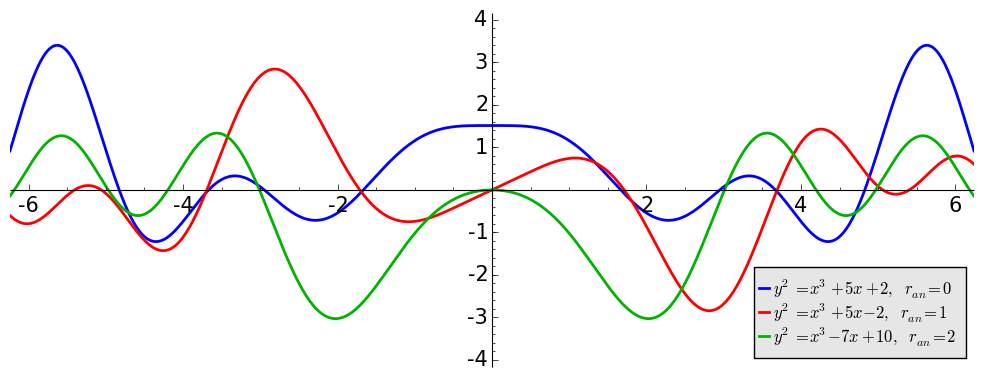
\includegraphics[width=1.0\textwidth]{graphics/L-functions_at_origin.png}
    \caption{The values of three elliptic curve L-functions along the critical line $1+it$ for $-6 \le t \le 6$. Blue corresponds to a rank 0 curve, red is that of a rank 1 curve, and green is a rank 2 curve. Note that close to the origin the graphs look like non-zero constant function, a straight line and a parabola respectively.}
    \label{fig:L-functions_at_origin}
\end{figure}

We can therefore at least conjecturally determine the curve's algebraic rank by computing the order of vanishing of the elliptic curve's $L$-function at the central point. This converts an generally difficult algebraic problem into a perhaps more tractable numerical one.

The work in this thesis hopes to address the question of how to effectively compute the order of vanishing of $L(E,s)$ at $s=1$, which is denoted $r_{an}$, the {\it analytic rank} of $E$. This, again, is a non-trivial task -- for example, how do you numerically determine if the $n$th Taylor coefficient of $L(E,s)$ is identically zero, or non-zero but so small that it is indistinguishable from zero given your finite-precision computations?

The short answer is that, for a black box computer, you can't. We need theorems governing the magnitude of the Taylor coefficients -- especially the leading coefficient $C$ in the BSD conjecture -- in order to make analytic rank explicitly computable. This work establishes those results, and details (assuming standard conjectures) an explicit algorithm with provable complexity to compute the analytic rank of a rational elliptic curve. \\

The structure of this dissertation is as follows. Chapter 2 more precisely lays out the problem tackled in this work, quotes the major results obtained to this end and outlines the strategy used to prove these results. Chapter 3 consists of an exposition of the mathematical background relevant to this thesis; while chapter 4 contains proofs of the main results. Chapter 5 is dedicated to supporting numerical data, and chapter 6 contains ancillary results, and ideas for future work.

\newpage
%%%%%%%%%%%%%%%%%%%%%%%%%%%%%%%%%%%%%%%%%%%%%%%%%%%%%%%%
\section{Problem Outline and Major Results}\label{sec:outline_results}

The central question this thesis addresses is thus: Given a rational elliptic curve $E$, does algorithm exist to compute the rank of $E$ that has provable worst-case and average-case running times? We answer this question in the affirmative; however, to do so we must pay the price of having to assume the three big open conjectures in number theory: The Generalized Riemann Hypothesis, The Birch and Swinnerton-Dyer conjecture, and the ABC conjecture (henceforth referred to as GRH, BSD and ABC respectively).

In this vein we establish the following results:

% QUOTE MAJOR RESULTS

\newpage
%%%%%%%%%%%%%%%%%%%%%%%%%%%%%%%%%%%%%%%%%%%%%%%%%%%%%%%%
section{Notation, Definitions and Background}\label{sec:defs_background}

%%%%%%%%%%%%%%%%%%%%%%%%%%
\subsection{Notation}

For the rest of the body of this text (unless otherwise stated) we use the following terminology:
\begin{itemize}
\item $E$ is an elliptic curve over $\QQ$ given by minimal Weierstrass equation $y^2 + a_1 xy + a_3 y^2 = x^3 + a_2 x^2 + a_4 x + a_6$, where $a_1, a_3 \in \set{0,1}$, $a_2 \in \set{-1,0,1}$ and $a_4,a_6 \in \ZZ$
\item $D$, $N$ and $r$ are the discriminant, conductor and algebraic rank of $E$ respectively
\item $r_{an}$ is the analytic rank of $E$
\item $p$ is a (rational) prime number and $q$ is a prime power
\item $s$ and $z$ are generic complex numbers
\item $\eta$ is the Euler-Mascheroni constant $= 0.5772156649\ldots$
\item $\gamma$ will always be used to denote the imaginary parts of nontrivial zeros of an $L$-function. \\
\end{itemize}

Furthermore, we define the following values associated to $E$ (in all cases the dependence on $E$ is understood):
\begin{itemize}
\item $b_2 = a_1^2 + 4a_2$
\item $b_4 = a_1 a_3 + 2a_4$
\item $b_6 = a_3^2 + 4a^6$
\item $b_8 = a_1^2 a_6 + 4 a_2 a_6 - a_1 a_3 a_4 + a_2 a_3^2 - a_4^2$
\item $c_4 = b_2^2 - 24 b_4$
\item $c_6 = -b_2^3 + 36 b_2 b_4  - 216 b_6$
\item $D = -b_2^2 b_8 - 8 b_4^3 - 27 b_6^2 + 9 b_2 b_4 b_6$; this is the definition of the discriminant of $E$
\item $j = \frac{c_4}{D}$
\item $\omega = \frac{dx}{2y + a_1 x + a_3} = \frac{dy}{3x^2 + 2a_2 x + a_4 - a_1 y}$
\end{itemize}

%%%%%%%%%%%%%%%%%%%%%%%%%%
\subsection{Definitions: Elliptic curves and their $L$-functions}

The rest of this chapter covers the basic definitions of and results surrounding elliptic curve $L$-functions. Feel free to skip this if you are familiar with them.

\begin{definition}
An elliptic curve $E$ is a genus 1 smooth projective curve with a marked point $\cO$. $E$ is defined over a field $K$ if $E$ may be represented by the {\it Weierstrass equation} $y^2 + a_1 xy + a_3 y^2 = x^3 + a_2 x^2 + a_4 x + a_6$, where $a1,\ldots a_6 \in K$.
\end{definition}

For elliptic curves defined over $\QQ$, we may always find a model for $E$ such that $a_1, a_3 \in \set{0,1}$, $a_2 \in \set{-1,0,1}$ and $a_4,a_6 \in \ZZ$. Furthermore, there is the notion of {\it minimality} when it comes to models for elliptic curves. Without going into the definition thereof, we will always assume that any given elliptic curve Weierstrass equation is minimal and in the above form, unless otherwise stated.

\begin{definition}
The set of $K$-rational points on $E$ is denoted $E(K)$. $E(K)$ comprises an abelian group, with the ``point at infinity" $\cO$ acting as the group identity element.
\end{definition}

It is often useful to view an elliptic curve $E$ as the vanishing locus of the polynomial
\begin{equation}\label{eqn:E_poly}
f(x,y) = y^2 + a_1 xy + a_3 y^2 - x^3 - a_2 x^2 - a_4 x - a_6.
\end{equation}
 That is $E(K) = \set{(x,y) \in K^2: \; f(x,y) = 0}$, along with the point at infinity $\cO$. \\

For a rational elliptic curve $E/\QQ$, we may consider the reduced curve $\tilde{E}/\Fp$ for any prime $p$. If $E/\QQ$ is given by $y^2 + a_1 xy + a_3 y^2 = x^3 + a_2 x^2 + a_4 x + a_6$, then for $p\ne 2$ or $3$ the reduced curve is given by $y^2 + \overline{a_1} xy + \overline{a_3} y^2 = x^3 + \overline{a_2} x^2 + \overline{a_4} x + \overline{a_6}$, where $\overline{a_i}$ is $a_i$ reduced modulo $p$. For $p = 2$ or $3$ we may have to move to a different model for $E$ first to avoid the reduced curve being automatically singular.

\begin{definition}
A prime $p$ is called {\it good} if $\tilde{E}/\Fp$ is non-singular. The reduced curve is an elliptic curve over $\Fp$ (by definition) which we denote by $E/\Fp$; $E$ is said to have {\it good reduction at $p$}. Otherwise, $p$ is said to be {\it bad}, the reduced (singular) curve is denoted $\tilde{E}/\Fp$, and $E$ is said to have {\it bad reduction at $p$}.
\end{definition}

\begin{theorem}
For any $E/\QQ$, the set of bad primes is finite and non-empty.
\end{theorem}

Singular reduced curves may be thought of as finite-field analogues of singular cubics over the rationals, for example those given by $y^2 = x^3$ and $y^2 = x^3+x^2$ as seen below. Singular curves have a (unique) {\it singular point}, which is by definition where the partial derivatives $\frac{\partial f}{\partial x}$ and $\frac{\partial f}{\partial y}$ are both zero (here $f$ is as given by equation \ref{eqn:E_poly}).

\begin{figure}[!h]
    \centering
    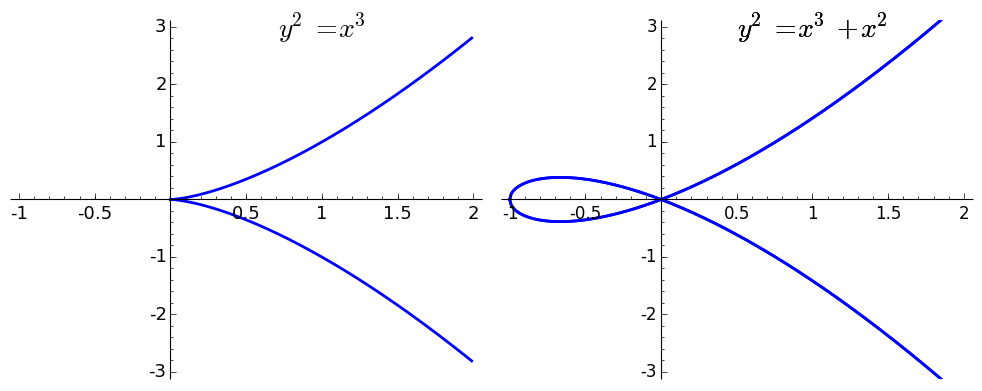
\includegraphics[width=1.0\textwidth]{graphics/singular_cubics.png}
    \caption{An example of two singular cubics over the rationals. The singular point for both curves is at the origin; for the the left curve the singular point is a {\it cusp}, and for the right curve it is a {\it node}.}
    \label{fig:singular_cubics}
\end{figure}

In the finite field setting the notion of partial derivatives still makes sense, so one may define singular points accordingly. Bad reduction at a prime may be classified into one of three types according to the nature of the tangent space at the singular point on $\tilde{E}/\Fp$.
\begin{definition}
Let $E$ have bad reduction at $p$; let $P$ be the singular point on $\tilde{E}/\Fp$, and let $T_P(E)$ be the tangent space at $P$.
\begin{itemize}
\item If the $T_P(E)$ is one-dimensional, then $P$ is a cusp, and $E$ is said to have {\it additive reduction} at $p$.
\item Otherwise $T_P(E)$ is two-dimensional, and $P$ is then a node; $E$ is then said to have {\it multiplicative reduction} at $p$. Furthermore, multiplicative reduction can be decomposed into two cases:
\begin{itemize}
\item If $T_P(E)$ is defined over $\Fp$, then $E$ is said to have {\it split multiplicative reduction} at $p$
\item Otherwise $T_P(E)$ is defined over a quadratic extension of $\Fp$, and $E$ is said to have {\it non-split multiplicative reduction} at $p$.
\end{itemize}
\end{itemize}
\end{definition}

Primes of bad reduction are packaged together into an invariant called the {\it conductor} of $E$:
\begin{definition}
The conductor of $E$, denoted by $N_E$ (or more often just $N$ when the choice of $E$ is unambiguous), is a positive integer given by
\begin{equation}
N_E = \prod_{p} p^{f_p(E)},
\end{equation}
where $p$ ranges over all primes, and for $p \ne 2$ or $3$,
\begin{equation}
f_p(E) = \begin{cases} 0, & \text{E has good reduction at $p$} \\ 1, & \text{E has multiplicative reduction at $p$} \\ 2, & \text{$E$ has additive reduction at $p$.}\end{cases}
\end{equation}
For $p=2$ and $3$, the exponent $f_p(E)$ is still zero if $p$ is good; however the exponent may be as large as $8$ and $5$ respectively if $p$ is bad.
\end{definition}
The ``proper" definition of the conductor is Galois representation-theoretic and is defined in terms of the representation of the inertia group at $p$ on the torsion subgroup of $E$; For $p\ne 2$ or $3$ this reduces to the definition given above, but for $2$ and $3$ there may be nontrivial wild ramification which increases the exponent up to the stated amounts. A full technical definition of the conductor is given in \cite[pp. 379-396]{Sil-1994}. In any case (including $2$ and $3$), the exponent $f_p(E)$ may be computed efficiently by Tate's algorithm, as detailed in the previous section of the same book \cite[pp. 361-379]{Sil-1994}. \\

We now move on to the definition of the $L$-function attached to an elliptic curve. For this we must define the numbers $a_p(E)$:
\begin{definition}\label{def:a_p} \mbox{}
\begin{itemize}
\item For good primes $p$ (i.e. when $p \nmid N$), let
\begin{equation}
a_p(E) = p+1-\#\set{\EFp},
\end{equation}
where $\#\set{\EFp}$ is the number of points on $E/\Fp$;
\item For bad primes (when $p \mid N$), let
\begin{equation}
a_p(E) := \begin{cases}
+1 & \text{if $E$ has split multiplicative reduction at $p$} \\
-1 & \text{if $E$ has non-split multiplicative reduction at $p$} \\
0 & \text{if $E$ has additive reduction at $p$.}
\end{cases}
\end{equation}
\end{itemize}
\end{definition}

Hasse's theorem states that the number of points on $E$ modulo $p$ can never be too far from $p+1$:
\begin{theorem}[Hasse, 1936]
For all elliptic curves $E/\QQ$ and all primes $p$,
\begin{equation}
|a_p(E)| \le \sqrt{p}
\end{equation}
\end{theorem}

For ease of notation, when $E$ is fixed we will let $a_p := a_p(E)$, letting the dependence on $E$ be understood. \\

The Sato-Tate Conjecture, now a theorem thanks to Taylor, goes even further, giving an asymptotic distribution on the $a_p$:
\begin{theorem}[Taylor, 2006-]
For fixed $E/\QQ$, the set of normalized $a_p$ values $\set{\frac{a_p}{2\sqrt{p}}: p \text{ prime}}$ obey a semicircular distribution on the interval $[-1,1]$. That is, for $1\le a \le b \le 1$, the asymptotic proportion of primes for which $a \le \frac{a_p}{2\sqrt{p}} \le b$ is equal to the proportion of the area under the unit semicircle between $a$ and $b$.
\end{theorem}

\begin{definition} \mbox{}

The $L$-function attached to $E$ is a complex analytic function $L_E(s)$, defined initially on some right half-plane of the complex plane.
\begin{itemize}
\item The Euler product of the $L$-function attached to $E$ is given by
\begin{equation}
L(E,s) = \prod_{p} \frac{1}{1 - a_p p^{-s} + \epsilon(p)p^{1-2s}}
\end{equation}
where $\epsilon(p) = 0$ for bad $p$, and $1$ for good $p$.
\item The Dirichlet series for $L_E(s)$ is given by
\begin{equation}
L(E,s) = \sum_{n=1}^{\infty} a_n n^{-s}.
\end{equation}
where for composite $n$, $a_n$ is defined to be the integer coefficient of $n^{-s}$ obtained by multiplying out the Euler product for $L(E,s)$.
\end{itemize}
\end{definition}
Again, we will often write $\Les$ or just $L(s)$ to simplify notation. \\

\begin{corollary} \mbox{}
\begin{itemize}
\item Hasse's Theorem implies that the Euler product and Dirichlet series for $\Les$ converge absolutely for $\Re(s) > \frac{3}{2}$.
\item Sato-Tate implies that the Euler product and Dirichlet series for $\Les$ converge conditionally for $\Re(s) > \frac{1}{2}$.
\end{itemize}
\end{corollary}

In this work we more often use the completed $L$-function attached to $E$:
\begin{definition}
The {\it completed $L$-function} attached to $E$ is given by
\begin{equation}
\Lambda_E(s) = N^{\frac{s}{2}}(2\pi)^{-s}\Gamma(s)\Les,
\end{equation}
where $N$ is the conductor of $E$ and $\Gamma(s)$ the usual Gamma function on $\CC$.
\end{definition}

Thanks to the modularity theorem, we may in fact analytically continue $\Les$ and $\Lams$ to be entire functions defined on all of $\CC$.
\begin{theorem}[Breuille, Conrad, Diamond, Taylor, Wiles et al, 1995,1999,2001] \mbox{}\\
There exists an integral newform $f = \sum_n a_n q^n$ of of weight $k=2$ and level $N$ such that $\Les = L_f(s)$.
\end{theorem}

The modularity theorem above is essentially the converse of the theorem by Shimura in the 1960s: if $f$ is a weight $2$ newform of level $N$, then there exists some elliptic curve $E/\Q$ of conductor $N$ such that $L_f(s) = L_E(s)$. Hence any theorem about elliptic curve $L$-functions is thus really a theorem about $L$-functions of weight 2 newforms in disguise. \\

\begin{corollary} \mbox{}
\begin{itemize}
\item $\Lams$ extends to an entire function on $\CC$. Specifically, $\Lams$ obeys the {\it functional equation}
\begin{equation}
\Lams = w_E \Lambda_E(2-s),
\end{equation}
where $w_E \in \set{-1, 1}$ is the action of the Atkin-Lehner involution on the newform attached to $E$.
\item $\Les$ extends to an entire function on $\CC$ via the definition of $\Lams$ and the functional equation above.
\end{itemize}
\end{corollary}

We reproduce the analytic continuation for $\Lams$ explicitly below. Define the auxiliary function $\lambda_E(s)$ by
\begin{equation}\label{eqn:Lams_analytic_continuation}
\lambda_E(s) = \left(\frac{\sqrt{N}}{2\pi}\right)^{s} \sum_{n=1}^\infty a_n n^{-s}\Gamma \left(s,\frac{2\pi n}{\sqrt{N}}\right),
\end{equation}
where all the quantities are as defined previously, and $\Gamma(s,x)$ is the upper incomplete Gamma function on $\CC\cross \RR_{>0}$. The sum converges absolutely for any $s$, so $\lambda_E(s)$ is entire. Then
\begin{equation}
\Lambda_E(s) = \lambda_E(s) + w_E \lambda_E(2-s)
\end{equation}
Knapp goes through the proof of this formula in \cite[pp. 270-271]{Kna-1992}. \\

\begin{definition}
$E$ is said to have {\it even parity} if $w_E = 1$, and {\it odd parity} if $w_E = -1$.
\end{definition}

The functional equation for $\Lams$ shows that it is either symmetric or antisymmetric about the line $\Re(s) = 1$; moreover, since all the constituent parts for $\Lams$ are defined over the reals, $\Lams$ is also conjugate symmetric about the real axis. It follows that $\Lams$ is highly symmetric about the point $s=1$. This is formalized in the following statement:
\begin{proposition}
As a function of $s$, $\Lambda_E(1+s)$ is even if $E$ has even parity, and odd if $E$ has odd parity.
\end{proposition}
This follows immediately from the functional equation. \\

We may use Equation \ref{eqn:Lams_analytic_continuation} to produce formulae for the value of $\Lams$ and its higher derivatives at $s=1$:
\begin{proposition} \mbox{}
\begin{enumerate}
\item \begin{equation}
\Lambda_E(1) = \begin{cases} \frac{\sqrt{N}}{\pi} \sum_{n=1}^{\infty}\frac{a_n}{n} e^{-\frac{2\pi}{\sqrt{N}}\cdot n}, & w_E = 1 \\ 0, & w_E = -1 \end{cases}
\end{equation}
\item When $k$ has the same parity as $E$, the $k$th derivative of $\Lams$ at the central point is given by
\begin{equation}\label{eqn:central_derivatives}
\Lambda_E^{(k)}(1) = 2 \sum_{n=1}^\infty a_n \int_{1}^{\infty} \left(\log \frac{t}{\sqrt{N}}\right)^k e^{-\frac{2\pi n}{\sqrt{N}}\cdot t} \; dx
\end{equation}
(when $k$ is opposite in parity to $E$, then $\Lambda_E^{(k)}(1) = 0$).
\end{enumerate}
\end{proposition}

\begin{proof}
Observe we may write equation \ref{eqn:Lams_analytic_continuation}, after a change of variables and swapping integration and summation signs, as
\begin{equation*}
\lambda_E(1+s) = N^{\frac{1+s}{2}}  \int_{\frac{1}{\sqrt{N}}}^{\infty} x^s f_E(it) \; dt  = N^{\frac{1+s}{2}}  \sum_{n=1}^\infty a_n \int_{\frac{1}{\sqrt{N}}}^{\infty} t^s e^{-2\pi nt} \; dt,
\end{equation*}
where $f_E$ is the cusp form attached to $E$. We may differentiate under the integral sign without issue and then evaluate at $s=1$ to get
\begin{equation*}
\lambda_E^{(k)}(1) = \sqrt{N}\cdot \sum_{n=1}^\infty a_n \int_{\frac{1}{\sqrt{N}}}^{\infty} (\log t)^k e^{-2\pi n t} \; dt
\end{equation*}
Equation \ref{eqn:central_derivatives} follows by substituting $t \mapsto \sqrt{N} \cdot t$. For $k=0$ the integrals may be evaluated directly: $\int_{1}^{\infty} e^{-\frac{2\pi n t}{\sqrt{N}}} \; dt = \frac{\sqrt{N}}{2\pi n} e^{-\frac{2\pi n}{\sqrt{N}}}$.
\end{proof}

\begin{definition} For elliptic curve $L$-functions:
\begin{itemize}
\item The point $s=1$ is called the {\it central point} or the {\it critical point}.
\item The vertical line of symmetry $\Re(s)=1$ is called the {\it critical line}.
\item The vertical strip $\frac{1}{2} \le \Re(s) \le \frac{3}{2}$ is call the {\it critical strip}.
\end{itemize}
\end{definition}

There is an oft-quoted anecdote that the way to differentiate analytic number theorists from algebraic number theorists is that for elliptic curve $L$-functions the former normalize so that the critical line lies at $\Re(s) = \frac{1}{2}$ (as is the case with $\zeta(s)$), while the latter keep the critical line at $\Re(s)=1$. In this thesis we work mostly with $L_E(1+s)$ and $\Lambda_E(1+s)$ which shifts the critical line to the imaginary axis; a move which is bound to antagonize both parties equally! \\

A standard result with $L$-functions of Hecke eigenforms (of elliptic curve $L$-functions are a subset) is that ``all the interesting stuff happens inside the critical strip'':
\begin{proposition}
$\Lambda_E(1+s) \ne 0$ for $|\Re(s)| > \frac{1}{2}$.
\end{proposition}
This can be proven by showing that the logarithmic derivative of $\Lambda_E(1+s)$ converges absolutely for $\Re(s) > \frac{1}{2}$. See section \ref{sec:log_derivs} for a proof (the statement can in fact be strengthened to asserting that all zeros are {\it strictly} inside the critical strip). \\

From the functional equation we get that $\Les$ has simple zeros at the nonpositive integers; these are denoted the {\it trivial} zeros of $\Les$. Zeros inside the critical strip are called {\it nontrivial}. The Generalized Riemann Hypothesis (stated in full in section \ref{sec:conjectures}) asserts that all nontrivial zeros of $\Les$ lie on the critical line $\Re(s)=1$, and all zeros with nonzero imaginary part are simple. 

If $\Les$ has a zero at the central point, it may or may not have multiplicity greater than 1. The multiplicity of this possible zero is denoted the analytic rank of $E$:
\begin{definition}
Let $E$ be an elliptic curve over $\Q$, and let $\Les$ be its $L$-series. The {\it analytic rank} of $E$, denoted $r_{an}(E)$ or just $r_{an}$ is the order of vanishing of $L_E(s)$ at the central point $s=1$. That is, if the Taylor series of $\Les$ about $s=1$ is
\begin{equation}
L_E(z) = a_0 + a_1 z + a_2 z^2 + \ldots
\end{equation}
where $z = s-1$, then $a_n = 0$ for $0 \le n < r_{an}$ and $a_{r_{an}} \ne 0$.
\end{definition}
We will work a lot with the leading coefficient of the $L$-seres at the central point, so it's worth giving it a name. To this end:
\begin{definition} \mbox{}
\begin{itemize}
\item Let $C^{\pr}_E$ (or just $C^{\pr}$ when $E$ is fixed) be the leading coefficient of $L_E(s)$ at the central point (the constant $a_{r_{an}}$ in the definition above)
\item Let $C_E$ (or just $C$ when $E$ is fixed) be the leading coefficient of $\Lams$ at the central point.
\end{itemize}
\end{definition}
Observe that $C_E = \frac{\sqrt{N}}{2\pi}\cdot C^{\pr}_E$. We will most often work with the former, hence the notation.

\newpage
%%%%%%%%%%%%%%%%%%%%%%%%%%%%%%%%%%%%%%%%%%%%%%%%%%%%%%%
\section{Some Conjectures}\label{sec:conjectures}

The main results in this thesis are contingent on the Birch and Swinnerton-Dyer conjecture, The Generalized Riemann Hypothesis and the ABC conjecture. We reproduce the three conjectures in full below. \\

The Birch and Swinnerton-Dyer conjecture (BSD) is needed to establish a way to compute and hence bound the magnitude of the leading coefficient of $\Les$ at the central point.
\begin{conjecture}[Birch, Swinnerton-Dyer]\label{conj:BSD}
\mbox{}
\begin{enumerate}
\item $r_{an} = r$; that is, the analytic rank of $E$ is equal to its algebraic rank.
\item The leading coefficient at the central point in $L_E(s)$ is given by
\begin{equation}
C_E^{\pr} = \left(\frac{\Omega_E\cdot\Reg_E\cdot\#\Sha(E/\Q)\cdot\prod_p c_p}{(\#E_{\text{Tor}}(\Q))^2}\right),\end{equation}
where
\begin{itemize}
\item $r$ is the algebraic rank of $E(\Q)$,
\item $\Omega_E$ is the real period of (an optimal model of) $E$,
\item $\Reg_E$ is the regulator of $E$,
\item $\#\Sha(E/\Q)$ is the order of the Shafarevich-Tate group attached to $E/\Q$,
\item $\prod_p c_p$ is the product of the Tamagawa numbers of $E$, and
\item $\#E_{\text{Tor}}(\Q)$ is the number of rational torsion points on $E$.
\end{itemize}
\end{enumerate}
\end{conjecture}

For an excellent description of the conjecture and a breakdown of the arithmetic invariants mentioned above, see Andrew Wiles' official description of the BSD Conjecture on the Clay Math website \cite{Wil-BSD}. \\

\begin{conjecture}[Generalized Riemann Hypothesis for Elliptic Curves, version 1]\label{conj:GRH1}
Let $E$ be an elliptic curve over $\Q$, and let $\Les$ be its $L$-series. If $\rho$ is a nontrivial zero of $\Les$ with nonzero imaginary part, then $\Re(\rho) = 1$. Moreover, all nontrivial noncentral zeros of $\Les$ are simple.
\end{conjecture}
That is, all nontrivial zeros of $\Les$ lie on the {\it critical line} $\Re(s)=1$, and the only place zeros can lie on top of each other is at the central point $s=1$. There are numerous equivalent formulations of GRH; we will most often use the following:
\begin{conjecture}[Generalized Riemann Hypothesis for Elliptic Curves, version 2]\label{conj:GRH2}
 \mbox{}
 Let $E$ be an elliptic curve over $\Q$, and let $\Lams$ be the completed $L$-function attached to $E$. Then
\begin{enumerate}
\item $\Lambda_E(1+s) = 0 \Longrightarrow \Re(s) = 0$.
\item $\Lambda_E(1+s) = 0$ and $\Lambda_E\pr(1+s) = 0 \Longrightarrow s=0$.
\end{enumerate}
\end{conjecture}

Finally, we will need strong form of the ABC conjecture of Masser and Oesterl\'{e} in order to establish lower bounds on the regulator and real period of $E$.
\begin{conjecture}[Masser-Oesterl\'{e}] \label{conj:ABC}
Let $(a,b,c)$ be a triple of coprime positive integers such that $a+b = c$, and let $\rad(abc) = \prod_{p | abc} p$ be the product of all primes dividing $a$, $b$ and $c$. Then for any $\epsilon > 0$ there is a constant $K_{\epsilon}$ such that
\begin{equation}
c < K_{\epsilon}\rad(abc)^{1+\epsilon}.
\end{equation}
\end{conjecture}
The ABC conjecture is famous for the large number of other results that it implies. Of these, we will need the following three that relate to elliptic curves:

\begin{conjecture}[Szpiro]\label{conj:Szpiro}
Let $E$ be an elliptic curve over $\QQ$ with conductor $N$ and minimal discriminant $D$. Then for any $\epsilon > 0$ there is a constant $K_{\epsilon}$ such that
\begin{equation}
|D| < K_{\epsilon}N^{6+\epsilon}.
\end{equation}
\end{conjecture}

\begin{conjecture}[Lang]\label{conj:Lang}
Let $E$ be an elliptic curve over $\QQ$ with minimal discriminant $D$. There is a positive constant $K$ such that for any nontorsion point $P\in E(\QQ)$,
\begin{equation}
\hat{h}(P) \ge K\log |D|,
\end{equation}
where $\hat{h}(P)$ is the N\'{e}ron-Tate canonical height of $P$.
\end{conjecture}

\begin{conjecture}[Hall]\label{conj:Hall}
For any $\epsilon > 0$ there is a constant $K_{\epsilon}$ such that for any $x,y \in \ZZ$ such that $x^3-y^2 \ne 0$, we have
\begin{equation}
|x^3-y^2| \ge K_{\epsilon} |x|^{\frac{1}{2}-\epsilon}.
\end{equation}
\end{conjecture}
That is, if $x^3-y^2 \ne 0$, then the difference cannot be closer than about $\sqrt{|x|}$.


\newpage
%%%%%%%%%%%%%%%%%%%%%%%%%%%%%%%%%%%%%%%%%%%%%%%%%%%%%%%%
\section{Logarithmic Derivatives}\label{sec:log_derivs}

Let $E/\QQ$  have conductor $N$.
\begin{definition}
The {\it logarithmic derivative} of the $L$-function attached to $E$ is
\begin{equation}
\ldLes := \frac{d}{ds} \log \Les = \frac{L_E^{\pr}(s)}{\Les}.
\end{equation}
\end{definition}
Logarithmic derivatives have some useful properties. Importantly, the logarithmic derivative of the product of meromorphic functions is the sum of the logarithmic derivatives thereof. To this end:
\begin{proposition}
\begin{equation}\label{eqn:logderiv_relation}
\ldLam{s} = \log\left(\frac{\sqrt{N}}{2\pi}\right) + \digamma(s) + \ldLe{s},
\end{equation}
where $\digamma(s) = \frac{\Gamma\pr}{\Gamma}(s)$ is the digamma function on $\C$.
\end{proposition}
This follows immediately from the definition of $\Lams = N^{\frac{s}{2}}(2\pi)^{-s}\Gamma(s)\Les$. \\

Note that the digamma function is well-understood and easily computable. For example, it has the following infinite sum expansion about $s=1$:
\begin{equation}\label{eqn:digamma_sum}
\digamma(1+s) = -\eta + \sum_{k=1}^{\infty} \frac{s}{k(k+s)}
\end{equation}
This series converges absolutely for any $s$ not equal to a negative integer, and uniformly on sets bounded away from the negative real axis.\\

What is perhaps surprising, however, is that $\ldLe{s}$ can be represented by an elegant Dirichlet series. Recall that for $p \nmid N$, the characteristic polynomial of Frobenius w.r.t.~$f$ at $p$ is $x^2 - a_p x + p^2$, where $a_p$ is as given by Definition \ref{def:a_p}. Let this quadratic polynomial split as $(x-\alpha_p)(x-\beta_p)$ in $\CC$, where for $\alpha_p$ and $\beta_p$ the dependance on $E$ is understood. \\

\begin{definition}\label{def:bn}
For $n \in \NN$, let
\begin{equation}
b_n(E) := \begin{cases}
-\left(\alpha_p^e+\beta_p^e\right)\cdot \log(p), & n=p^e\;\;\text{a prime power ($e\ge1$), and $p \nmid N$} \\
-a_p^e \cdot \log(p), & n=p^e\;\;\text{and $p \mid N$} \\
0, & \text{otherwise,} \end{cases}
\end{equation}
\end{definition}

\begin{lemma}
The Dirichlet series for $\ldLes$ is given by
\begin{equation}
\ldLes = \sum_{n=1}^{\infty} b_n(E)\, n^{-s}
\end{equation}
where the coefficients $b_n(E)$ are defined as in Definition \ref{def:bn}. \\
\end{lemma}
\begin{proof}
The proof is an exercise in taking the logarithmic derivative of the Euler product formula for $\Les$ and simplifying. Note we may write the Euler product of $\Les$ as
\begin{equation}
\Les = \prod_{p|N} \left(1-a_p p^{-s}\right)^{-1} \prod_{p\nmid N} \left(1-\alpha_p p^{-s}\right)^{-1}\left(1-\beta_p p^{-s}\right)^{-1}.
\end{equation}
The result follows by taking the logarithmic derivative of each term individually and then summing the results.
\end{proof}

The Dirichlet coefficients for $\ldLes$ have a beautiful characterization in terms of the number of points on $E$ over finite fields:
\begin{theorem}[S.]
\begin{equation}
b_n(E) = \begin{cases}
-\left(p^e + 1 - \#\widetilde{E}(\FF_{p^e})\right)\cdot \log(p), & n=p^e\;\;\text{a prime power,} \\
0, & \text{otherwise} \end{cases}
\end{equation}
where $\#\widetilde{E}(\FF_{p^e})$ is the number of points over $\FF_{p^e}$ on the (possibly singular) curve obtained by reducing $E$ modulo $p$.
\end{theorem}

\begin{proof}
It is a standard result that if $(x-\alpha_p)(x-\beta_p)$ is the characteristic polynomial for Frobenius on $E$ at prime $p$ of good reduction, then
\begin{equation}
\#E(\FF_{p^e}) = p^e + 1 - \alpha_p^e - \beta_p^e
\end{equation}
(see \cite[pp. 134-136]{Sil-1985} for a proof), from which the result at $p \nmid N$ follows. \\

For primes of bad reduction, recall
\begin{equation}
a_p(E) := \begin{cases}
+1, & \text{$E$ has split multiplicative reduction at $p$} \\
-1, & \text{$E$ has non-split multiplicative reduction at $p$} \\
0, & \text{$E$ has additive reduction at $p$}
\end{cases}
\end{equation}
Let $\Ensfpe$ be the group of nonsingular points on $\widetilde{E}(\FF_{p^e})$. \\
When $E$ has additive reduction at $p$, $\Ensfpe \simeq (\F_{p^e},+)$, so together with the singular point $\#\widetilde{E}(\FF_{p^e}) = p^e+1$; \\
Hence $(p^e + 1 - \#\widetilde{E}(\FF_{p^e}))\log(p) = 0 = a_p^e \log(p)$. \\
When $E$ has split multiplicative reduction at $p$, $\Ensfpe \simeq (\F_{p^e}^*,\times)$, so together with the singular point $\#\widetilde{E}(\FF_{p^e}) = (p^e-1)+1 = p^e$; So $(p^e + 1 - \#\widetilde{E}(\FF_{p^e}))\log(p) = 1\cdot \log(p) = a_p^e \log(p)$. \\
When $E$ has non-split multiplicative reduction at $p$, let $L/\FF_{p^e}$ be the quadratic extension obtained by adjoining to $\FF_{p^e}$ the slopes of the tangent lines  at the singular point; then $\Ensfpe \simeq \ker(\Norm_{L/\FF_{p^e}})$. \\
Some thought should convince you that there are $p^e-(-1)^e$ elements in $L$ with norm 1, so together with the singular point $\#\widetilde{E}(\FF_{p^e}) = p^e+1-(-1)^e$; \\
Hence $(p^e + 1 - \#\widetilde{E}(\FF_{p^e}))\log(p) = (-1)^e\cdot \log(p) = a_p^e \log(p)$.
See \cite[pg. 180, Prop. 5.1]{Sil-1985} for the proofs of the above isomorphisms.\\
\end{proof}

With elliptic curve $L$-functions it is often easier to work with the shifted logarithmic derivative $\ldLe{1+s}$ as it places the critical point at the origin. We therefore define notation for the coefficients of the shifted Dirichlet series below:
\begin{definition}\label{def:cn}
The logarithmic derivative of the shifted $L$-function $L_E(1+s)$ is given by Dirichlet series
\begin{equation}
\ldLe{1+s} := \sum_n c_n n^{-s} = \sum_{n} \frac{b_n}{n} n^{-s},
\end{equation}
i.e. $c_n = b_n/n$, where the $b_n$ are as defined in Definition \ref{def:bn}.
\end{definition}

Because of its transparent Dirichlet series, we can bound the magnitude of $\ldLe{1+s}$ for $\Re(s)>\frac{1}{2}$. Let $\frac{\zeta\pr}{\zeta}$ be the logarithmic derivative of the Riemann zeta function. Then $\frac{\zeta\pr}{\zeta}(s) = \sum -\lambda(n) n^{-s}$ for $\Re(s)>1$, where $\lambda(n)$ is the von Mangoldt function, given by
\begin{equation}\label{eqn:vonmangoldt}
\lambda(n) = \begin{cases} \log p & n = p^e \;\;\text{a perfect prime power,} \\ 0 & \text{otherwise.} \end{cases}
\end{equation}
Observe that $-\frac{\zeta\pr}{\zeta}(s)$ is strictly positive for $s > 1$ real and decays to zero exponentially as $s \to \infty$. \\

Away from the critical strip the behavior of $\Les$ is tightly constrained.
\begin{lemma}\label{lem:ldLe_bound}
Let $E$ be an elliptic curve $L$-function $L_E(s)$. For $\Re(s)>\frac{1}{2}$ we have\begin{equation}
2\frac{\zeta\pr}{\zeta}\left(\frac{1}{2}+\Re(s)\right) < \left| \ldLe{1+s}\right| < -2\frac{\zeta\pr}{\zeta}\left(\frac{1}{2}+\Re(s)\right).
\end{equation}
\end{lemma}

\begin{proof}
Let $\sigma = \Re(s)$. By Hasse's Theorem we have that $|q + 1 - \#\widetilde{E}(\FF_{q})| \le 2\sqrt{q}$ for any prime power $q$. Hence
\begin{align*}
\left| \ldLe{1+s}\right| &\le \sum_n \frac{|b_n|}{n} n^\sigma < \sum_{n} \frac{2\sqrt{n} \cdot \lambda(n)}{n} n^{-\sigma}  = -2\frac{\zeta\pr}{\zeta}\left(\frac{1}{2}+\sigma\right).
\end{align*}
The inequality in the middle is strict, as Hasse's bound cannot be hit when $n$ is prime. The left inequality is proved in the same way with the signs reversed.
\end{proof}
Note that these bounds are global: they do not depend on the elliptic curve $E$ in any way.

\begin{corollary}
$\Lambda_E(1+s)$ has no zeros outside the critical strip $|\Re(s)| \le \frac{1}{2}$.
\end{corollary}
\begin{proof}
Recall that if $f$ is meromorphic on $\CC$, then $\frac{f\pr}{f}$ has a pole at $s=s_0$ iff $f$ has a zero or pole at $s_0$; moreover poles of $\frac{f\pr}{f}$ are simple and have residue equal to the multiplicity of the corresponding zero/pole of $f$. But by the above $\ldLe{1+s}$ converges absolutely for $\Re(s)>\frac{1}{2}$, so $\ldLam{1+s}$ is well-defined and bounded for $\Re(s)>\frac{1}{2}$, and hence cannot have any poles in this region. By symmetry the same is true for $\Re(s)<-\frac{1}{2}$. Hence $\Lambda_E(1+s)$ cannot have any zeros for $|\Re(s)| > \frac{1}{2}$.
\end{proof}

$\Lambda_E(1+s)$ has a particularly simple representation as a product over its zeros, from which we get a representation of $\ldLam{1+s}$ as a sum over its zeros.
\begin{lemma}  \mbox{}
\begin{enumerate}
\item \begin{equation}\label{eqn:Lams_prod}
\Lambda_E(1+s) = C_E\cdot r_{an}^s \cdot \prod_{\gamma > 0} \left(1+\frac{s^2}{\gamma^2}\right) 
\end{equation}
where $C_E$ is the leading coefficient of $\Les$ at the central point (i.e. that defined in Conjecture \ref{conj:BSD}), and the product is taken over all zeros of $\Lambda_E(1+s)$ in the upper half plane. The product converges absolutely for any $s$, and uniformly on any bounded set.
\item \begin{equation}\label{eqn:ldLam_sum}
\ldLam{1+s} = \sum_{\gamma} \frac{s}{s^2+\gamma^2}, 
\end{equation}
where the sum is taken over {\bf all} nontrivial zeros of $\Lambda_E(1+s)$ (including central zeros) with multiplicity. The sum converges absolutely for any $s$ outside the set of nontrivial zeros for $L_E(1+s)$, and uniformly on any bounded set. \\
\end{enumerate}
\end{lemma}

Note that if we assume GRH (as we always do), then $\gamma^2$ is always a nonnegative real number in any of the above expansions. Furthermore,  since noncentral nontrivial zeros occur in conjugate pairs, each term for $\gamma \ne 0$ in Equation \ref{eqn:ldLam_sum} appears exactly twice. It is therefore often useful to rewrite it as
\begin{equation}\label{eqn:ldLam_sum_v2}
\ldLam{1+s} = \frac{r_{an}}{s} + 2 \sum_{\gamma>0} \frac{s}{s^2+\gamma^2}.
\end{equation}

\begin{proof}
Observe that $\Lambda_E(1+s)$ has a zero of order $r_{an}$ at the origin, and by GRH all other zeros of $\Lambda_E(1+s)$ are simple, lie on the imaginary axis, and are symmetric about the origin. \\

Now since $\Lambda_E(1+s)$ is an entire function of finite order, we may express it as a Hadamard product over its zeros. As with the Hadamard product for the completed Riemann Zeta function, the symmetry of $\Lambda_E(1+s)$ simplifies this product to
\begin{equation}
\Lambda_E(1+s) = C_E s^{r_{an}}\prod_{\gamma\ne0}\left(1-\frac{s}{i\gamma}\right),
\end{equation}
where $C_E$ is the leading nonzero coefficient of the Taylor series for $\Lambda_E(1+s)$ at the central point; and for convergence the product should be taken over conjugate pairs of zeros. Combining conjugate pair terms yields Equation \ref{eqn:Lams_prod}; logarithmic differentiation then yields Equation \ref{eqn:ldLam_sum_v2}, which can be simplified to Equation \ref{eqn:ldLam_sum}.
\end{proof}

\begin{corollary}
$\ldLam{1+s}$ is an odd function.
\end{corollary}

The following corollary will be of import in obtaining explicit bounds on the number of zeros of $L_E(s)$ in a given interval on the critical strip:
\begin{corollary}\label{cor:Re_logderiv}
Let $\Re(s) > 0$, and write $s = \sigma + i\tau$, i.e. $\sigma > 0$. Then
\begin{equation}
\sum_{\gamma} \frac{\sigma}{\sigma^2+(\gamma-\tau)^2} = \Re\left(\ldLam{1+s}\right),
\end{equation}
where again the sum is taken over all nontrivial zeros of $L_E(s)$. The sum converges absolutely for any $\tau \in \RR$ and $\sigma > 0$.
\end{corollary}
\begin{proof}
By equation \ref{eqn:ldLam_sum} we have
\begin{align*}
\Re\left(\ldLam{1+s}\right) &= \Re\left(\sum_{\gamma} \frac{s}{s^2+\gamma^2}\right) \\
& = \frac{1}{2} \sum_{\gamma} \Re\left(\frac{1}{s - i \gamma} + \frac{1}{s + i \gamma}\right) \\
&= \frac{1}{2} \sum_{\gamma} \frac{\sigma}{\sigma^2+(\gamma-\tau)^2} +  \frac{\sigma}{\sigma^2+(\gamma+\tau)^2}
\end{align*}
However, absolute convergence for $\sum_{\gamma} \frac{s}{s^2+\gamma^2}$ for any $s$ in the right half plane implies absolute convergence for the individual sums $\sum_{\gamma} \frac{\sigma}{\sigma^2+(\gamma-\tau)^2}$ and $\sum_{\gamma} \frac{\sigma}{\sigma^2+(\gamma+\tau)^2}$. We may thus write
\begin{align*}
\Re\left(\ldLam{1+s}\right) &= \frac{1}{2} \sum_{\gamma} \frac{\sigma}{\sigma^2+(\gamma-\tau)^2} +  \frac{1}{2} \sum_{\gamma}\frac{\sigma}{\sigma^2+(\gamma+\tau)^2} \\
&= \sum_{\gamma} \frac{\sigma}{\sigma^2+(\gamma-\tau)^2} \;\;\text{by symmetry.}
\end{align*}
\end{proof}
Observe that GRH implies that $\Re(\ldLam{1+s})>0$ for $\Re(s)>0$, since then each of the terms in the above sum are strictly positive. By oddness of $\ldLam{1+s}$ we also then have that $\Re(\ldLam{1+s})<0$ for all $\Re(s)<0$, and $\Re(\ldLam{1+s})=0 \Rightarrow \Re(s)=0$. \\

Mazur and Stein in \cite{MaSt-2013} define the {\it bite} of an elliptic curve $L$-function:
\begin{definition}
The {\it bite} of $\Les$ is
\begin{equation}
\beta(E) := \sum_{\gamma \ne 0} \gamma^{-2},
\end{equation}
where the sum runs over the imaginary parts of all {\it noncentral} nontrivial zeros of $\Les$.
\end{definition}
This quantity ends up controlling the rate of convergence in many of the sums that appear in explicit formula-type relations for $\Les$. Again, the explicit dependence on $E$ may be left as understood if the choice of $E$ is unambiguous.

Since sums of inverse higher powers of zeros also crop up, we generalize the notion of bite as follows:
\begin{definition}
For positive integer $n$, the {\it higher order bite} of order $n$ for $\Les$ is
\begin{equation}
\beta_n(E) := \sum_{\gamma \ne 0} \gamma^{-n}.
\end{equation}
\end{definition}
Thus $\beta_2(E) = \beta(E)$ as defined previously. Note also that $\beta_n = 0$ for any odd $n$, since zeros come in conjugate pairs. \\

Equation \ref{eqn:ldLam_sum} gives us a description of the Laurent expansion of $\ldLam{1+s}$ about zero:
\begin{corollary}\label{cor:ldLam_series_at_zero}
The Laurent expansion of $\ldLam{1+s}$ about zero is given by
\begin{align}
\ldLam{1+s} &= \frac{r_{an}}{s} + \beta_2(E) s - \beta_4(E) s^3 + \beta_6(E) s^5 - \ldots \\
& = \frac{r_{an}}{s} + \sum_{k=1}^{\infty} \left[(-1)^{k-1}\beta_{2k}(E)\right] s^{2k-1}
\end{align}
and this converges for $|s|<\gamma_0$, where $\gamma_0$ is the imaginary part of the lowest noncentral nontrivial zero of $\Les$ in the upper half plane.
\end{corollary}
The proof of this follows immediately by expanding the sum in Equation \ref{eqn:ldLam_sum} and collecting terms. \\

\begin{corollary}\label{cor:ldLe_expansion}
Let $E/\QQ$ have conductor $N$, $L$-function $\Les$ and bite $\beta = \beta_2(E)$. Let the Taylor series expansion of $L_E$ about the central point be
\begin{equation}
L_E(1+s) = Cs^{r_{an}}\left[1 + a\cdot s + b\cdot s^2 + O(s^3)\right]
\end{equation}
Then 
\begin{align}
a &= -\left[-\eta + \log\left(\frac{\sqrt{N}}{2\pi}\right)\right] \\
2b &= \left[-\eta + \log\left(\frac{\sqrt{N}}{2\pi}\right)\right]^2 - \frac{\pi^2}{6} + \beta,
\end{align}
where $\eta$ is the Euler-Mascheroni constant $= 0.5772\ldots$.
\end{corollary}

\begin{proof}
We note that the digamma function has the following Taylor expansion about $s=1$:
\begin{equation}
\digamma(1+s) = -\eta - \sum_{k=1}^{\infty} (-1)^k \zeta(k+1) s^k,
\end{equation}
where $\eta$ is the Euler-Mascheroni constant, and $\zeta(s)$ is the Riemann zeta function. \\
Thus by equation \ref{eqn:logderiv_relation} and Corollary \ref{cor:ldLam_series_at_zero} we have that
\begin{equation*}
\ldLe{1+s} = \frac{r_{an}}{s} - \left[-\eta + \log\left(\frac{\sqrt{N}}{2\pi}\right)\right] + \left[-\zeta(2) + \sum_{\gamma\ne0} \gamma^{-2}\right]\cdot s + O(s^2)
\end{equation*}
But if $L_E(1+s) = Cs^{r_{an}}\left[1 + a\cdot s + b\cdot s^2 + O(s^3)\right]$, then careful logarithmic differentiation yields
\begin{equation*}
\ldLe{1+s} = \frac{r_{an}}{s} + a + \left(-a^2 + 2b\right)\cdot s + O(s^2)
\end{equation*}
Comparing terms and solving for the relevant quantities produces the desired formulae.
\end{proof}
We may continue in the same vein to produce formulae for higher order coefficients of $L_E(s)$. As can be seen from above, these can in general be written in terms of sums of powers of $\left[-\eta + \log\left(\frac{\sqrt{N}}{2\pi}\right)\right]$, inverse sums of even powers of the nontrivial zeros, and $\zeta(n)$ for $n$ a positive integer. \\

What's also worth pointing out here is that the above suggests that the Taylor expansion about $s=1$ of the $L$-series attached to $E$ essentially contains no new information about the curve's attached invariants beyond that which can be found in the first nonzero coefficient - unless that information is somehow encoded in the bites $\beta_{2n}(E)$ for $n \in \NN$. Whether this is the case or not, however, is an open question.


\newpage
%%%%%%%%%%%%%%%%%%%%%%%%%%%%%%%%%%%%%%%%%%%%%%%%%%%%%%%
\section{Zero Sums and the Explicit Formula}

Combining equations \ref{eqn:logderiv_relation}, \ref{eqn:digamma_sum} and \ref{eqn:ldLam_sum} we get the following equality:
\begin{proposition}
Let $E/\QQ$ have conductor $N$. Let $\gamma$ range over all nontrivial zeros of $\Les$ with multiplicity, let $\eta$ be the Euler-Mascheroni constant, and let the $c_n = c_n(E)$ be as given by definitions \ref{def:bn} and \ref{def:cn}. Then
\begin{equation}\label{eqn:exp_form_1}
\sum_{\gamma} \frac{s}{s^2 + \gamma^2} = \left[-\eta + \log\left(\frac{\sqrt{N}}{2\pi}\right)\right] + \sum_{k=1}^{\infty} \frac{s}{k(s+k)} + \sum_{n=1}^{\infty} c_n n^{-s}
\end{equation}
\end{proposition}
This is the prototypical {\it explicit formula} for elliptic curves: an equation relating a sum over the nontrivial zeros of $\Les$ to a sum over the logarithmic derivative coefficients of $\Les$, plus some easily smooth part that only depends on the curve's conductor. \\

In general, the phrase ``explicit formula" is not applied to a specific equation, but rather to a suite of formula that resemble the above in some way. We reproduce lemma 2.1 from \cite{Bob-2011}, which is a more general version of the explicit formula, akin to the Weil formulation of the Riemann-von Mangoldt explicit formula for $\zeta(s)$.
\begin{lemma}\label{lem:exp_form_2}
Suppose that $f(z)$ is an entire function s.t. there exists a $\delta>0$ such that $f(x+iy) = O(x^{-(1+\delta)})$ for $|y|<1+\epsilon$ for some $\epsilon>0$. Suppose that the Fourier transform of $f$
\begin{equation}
\hat{f}(y) = \int_{-\infty}^{\infty} e^{-i x y}f(x)\; dx
\end{equation}
exists and is such that $\sum_{n=1}^{\infty} c_n \hat{f}\left(\log n\right)$ converges absolutely. Then
\begin{equation}\label{eqn:exp_form_2}
\sum_{\gamma} f(\gamma) = \frac{1}{\pi}\left[\log\left(\frac{\sqrt{N}}{2\pi}\right)\hat{f}(0) + \Re\int_{-\infty}^{\infty} \digamma(1+it)f(t) \; dt  + \frac{1}{2} \sum_{n=1}^{\infty} c_n \left( \hat{f}\left(\log n\right) + \hat{f}\left(-\log n\right)\right) \right]
\end{equation}
\end{lemma}
A proof can be found in \cite[Theorem 5.12]{IwKo-2004}. Note that Equation \ref{eqn:exp_form_1} can be recovered by setting $f$ to be the Poisson kernel $f_s(x) = \frac{s}{s^2+x^2}$; then $\hat{f_s}(y) = e^{-s|y|}$, so $\hat{f_s}(\log n) = n^{-s}$. \\

We give a distribution-theoretic reformulation of Lemma \ref{lem:exp_form_2}. While the subject of explicit formulae for $L$-functions of Hecke eigenforms is treated by a number of sources, the following doesn't seem to have been explicitly written down in the literature anywhere:
\begin{proposition}[S.]
Let $\gamma$ range over the imaginary parts of the zeros of $\Les$ with multiplicity. Let $\varphi_E = \sum_{\gamma} \delta(x-\gamma)$ be the complex-valued distribution on $\RR$ corresponding to summation over the zeros of $L_E(s)$, where $\delta(x)$ is the usual Dirac delta function. That is, for any test function $f: \RR \mapsto \CC$ such that $\sum_{\gamma}f(\gamma)$ converges, 
\begin{equation}
\langle f,\varphi_E \rangle = \int_{-\infty}^{\infty} f(x)\left(\sum_{\gamma\in S_E} \delta(x-\gamma)\right) \, dx = \sum_{\gamma\in S_E} f(\gamma).
\end{equation}
Then as distributions,
\begin{equation}\label{eqn:exp_form_3}
\varphi_E = \sum_{\gamma} \delta(x-\gamma) = \frac{1}{\pi}\left[-\eta + \log\left(\frac{\sqrt{N}}{2\pi}\right) +\sum_{k=1}^{\infty} \frac{x^2}{k(k^2+x^2)} + \frac{1}{2}\sum_{n=1}^{\infty} c_n \left(n^{ix}+n^{-ix}\right) \right].
\end{equation}
\end{proposition}
In the above language, $\ldLam{1+s} = \left\langle \frac{s}{s^2+x^2},\varphi_E \right\rangle$ for $\Re(s) > 0$. Note that convergence on the right hand side is absolute for $\Re(s)>1$, and conditional (provably so thanks to Sato-Tate) for $0<\Re(s)\le 1$. \\

\newpage
%%%%%%%%%%%%%%%%%%%%%%%%%%%%%%%%%%%%%%%%%%%%%%%%%%%%%%%
\section{The Distribution of Nontrivial Zeros}

\begin{definition}
For non-negative $t$, let $M_E(t)$ be the modified non-trivial zero counting function for $\Les$, i.e.
\begin{equation}
M_E(t) := \sideset{}{\pr}\sum_{|\gamma| \le t} \frac{1}{2}
\end{equation}
where $\gamma$ runs over the imaginary parts of nontrivial zeros of $L_E(s)$, and the prime indicates that the final $\gamma$ is taken with half weight if $\gamma = t$. The central zero is taken with with multiplicity $r$, where $r$ is the analytic rank of $E$. \\
\end{definition}

Note that $M_E(0) = \frac{r}{2}$, and the function jumps by 1 across the locations of nontrivial zeros, since noncentral zeros come in conjugate pairs and (by GRH) are always simple. \\

\begin{proposition}[S.]
\begin{equation}\label{eqn:M_E(t)}
M_E(t) = \frac{1}{\pi}\left[\left(-\eta+\log\left(\frac{\sqrt{N}}{2\pi}\right)\right) t + \sum_{k=1}^{\infty} \left(\frac{t}{k} - \arctan\left(\frac{t}{k}\right)\right) + \sum_{n=1}^{\infty} \frac{c_n}{\log n}\cdot \sin(t\log n)\right]
\end{equation}
Convergence on the RHS is pointwise with respect to $t$ for both sums; for fixed $t$ convergence for the sums over $k$ and $n$ is absolute and conditional respectively (and {\it extremely} slow for the latter).
\end{proposition}

\begin{proof}
Observe we may write $M_E(t) = \sum_{\gamma}f_t(\gamma)$, where
\begin{equation}
f_t(x) = \begin{cases} \frac{1}{2}, & |x|<t \\ \frac{1}{4}, & |x| = t \\ 0 & |x|> t \end{cases}
\end{equation}
Informally, we obtain the above formula by integrating both sides of Equation \ref{eqn:exp_form_3} against $f = f_t(x)$, noting that $\hat{f}_t(y) = \frac{\sin(ty)}{y}$. The integrals in the sum over $k$ give us no issue and we may swap the order of the integral and summation signs, since convergence there is absolute. However, some care must be taken when it comes to the sum over $n$, since here convergence is only conditional. 

Formally, we must write $M_E(t)$ as a path integral of $\ldLam{1+s}$ on the path
\begin{equation*}
\epsilon-it \mapsto \epsilon+it \mapsto -\epsilon+it \mapsto -\epsilon-it \mapsto \epsilon-it
\end{equation*}
for some $\epsilon>0$, and invoke the Cauchy Residue Theorem. We may then shrink $\epsilon$ to zero (assuming GRH) to obtain that the RHS of \ref{eqn:M_E(t)} converges point wise to $M_E(t)$ as $m$ and $n \to \infty$.
\end{proof}

Equation \ref{eqn:M_E(t)} may be though of having two components. The first two terms comprise a smooth part that gives the ``expected number of zeros'' up to $t$; and the trigonometric sum over $n$ comprises the discretization information that yields the zeros' exact locations. We expect the trigonometric sum to be zero infinitely often, and asymptotically it should be positive as often as it is negative. As such the sum should average out to zero and shouldn't contribute any asymptotic bias to the density of zeros on the critical line. We can therefore talk in a real sense of the expected number of zeros up to $t$, which is given by
\begin{equation}\label{eqn:M_E_smooth_part}
\frac{1}{\pi}\left[\left(-\eta+\log\left(\frac{\sqrt{N}}{2\pi}\right)\right) t + \sum_{k=1}^{\infty} \left(\frac{t}{k} - \arctan\left(\frac{t}{k}\right)\right)\right]
\end{equation}

Moreover, the trigonometric sum should grow very slowly with $t$. Put more formally, we have the following:
\begin{conjecture}\label{conj:trig_sum_size}
\begin{equation}
\sum_{n=1}^{\infty} \frac{c_n}{\log n}\cdot \sin(t\log n) = O(\log t)
\end{equation}
\end{conjecture}
This statement should follow from GRH, and is borne out by numerical evidence:

\begin{figure}[!h]
    \centering
    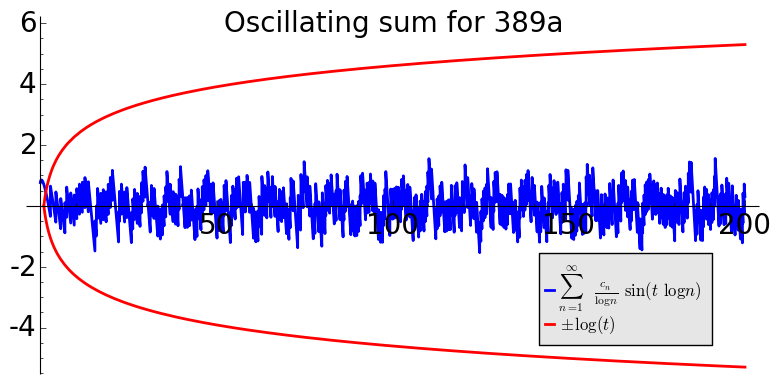
\includegraphics[width=1.0\textwidth]{graphics/M_E_trig_sum_bounds.png}
    \caption{The oscillating sum $\sum_{n=1}^{\infty} \frac{c_n}{\log n}\cdot \sin(t\log n)$ for the curve with Cremona label $389a$ (with equation $y^2 + y = x^3 + x^2 - 2x$) versus $\pm \log(t)$ for $0\le t \le 200$. Numerically we actually see the maximum value of the sum grow slower than $\log(t)$ - possibly $\log(t)^{\alpha}$ for some $0<\alpha<1$, or even $\log\log(t)$.}
    \label{fig:M_E_trig_sum_bounds}
\end{figure}

\begin{lemma}\label{lem:arctan_sum_size}
For $t >> 0$, 
\begin{equation}
\sum_{k=1}^{\infty} \left(\frac{t}{k} - \arctan\left(\frac{t}{k}\right)\right) = t\log t + (\eta-1)t + \frac{\pi}{4} + O\left(\frac{1}{t}\right),
\end{equation}
where $\eta = 0.5772\ldots$ is the Euler-Mascheroni constant.
\end{lemma}
\begin{proof}
We have
\begin{equation*}
\sum_{k=1}^{\infty} \left(\frac{t}{k} - \arctan\left(\frac{t}{k}\right)\right) = \int_{0}^{t} \sum_{k=1}^{\infty} \frac{x^2}{k(k^2+x^2)} \; dx = \int_{0}^{t} \Re\left(\digamma(1+ix) + \eta\right) \; dx,
\end{equation*}
where $\digamma(z)$ is the digamma function on $\CC$. Now along the critical line we have the following asymptotic expansion for the real part of the digamma function:
\begin{equation}
\Re\left(\digamma(1+ix)\right) = \log x + \frac{1}{12} x^{-2} + O(x^{-4})
\end{equation}
Hence $\int_{0}^{t} \Re\left(\digamma(1+ix)\right) \; dx = t(\log t - 1)  + O(1)$. The constant term of $\frac{\pi}{4}$ comes from integrating the difference between $\Re\left(\digamma(1+ix)\right)$ and $\log x$ between $0$ and $\infty$:
\begin{equation*}
\int_{0}^{\infty} \left[\Re\left(\digamma(1+ix)\right) - \log x\right] \; dx = \frac{\pi}{4}.
\end{equation*}
The result follows.
\end{proof}

Conjecture \ref{conj:trig_sum_size} and lemma \ref{lem:arctan_sum_size} combine to give us a precise asymptotic statement on the distribution of zeros up to $t$, in the same vein as von Mangoldt's asymptotic formula for the number of zeros up to $t$ for $\zeta$:

\begin{theorem}[S.]\label{thm:zero_density}
Let $E$ have conductor $N$. Then for $t>>0$ we have
\begin{equation}
M_E(t) = \frac{t}{\pi}\left[\log\left(\frac{t\sqrt{N}}{2\pi}\right) -1 \right] + \frac{1}{4} + O(\log t),
\end{equation}
where the error term is positive as often as it negative and contributes no net bias.
\end{theorem}

\begin{figure}[!h]
    \centering
    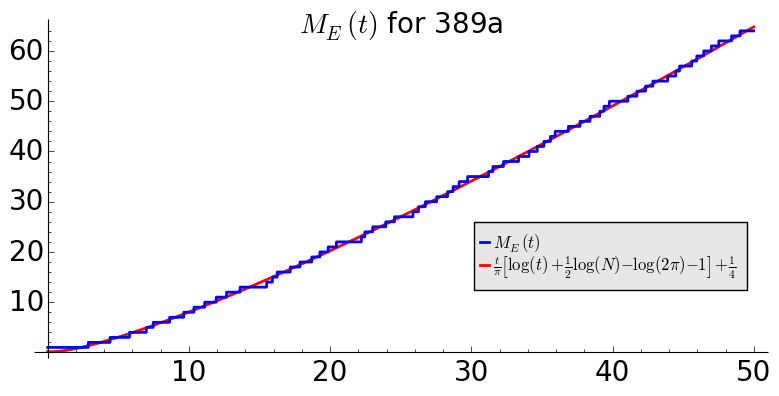
\includegraphics[width=1.0\textwidth]{graphics/M_E_389.png}
    \caption{The number of zeros up to $t$ versus $\frac{t}{\pi}\left[\log\left(\frac{t\sqrt{N}}{2\pi}\right) -1 \right] + \frac{1}{4}$ for the Cremona curve $389a$. The match up is extremely good.}
    \label{fig:M_E_389}
\end{figure}

\begin{corollary}
For $t>>0$, the number of zeros on the critical line in a unit interval
\begin{equation}
M_E(t)-M_E(t-1) = \frac{1}{\pi}\log\left(\frac{t\sqrt{N}}{2\pi}\right) + O(\log t),
\end{equation}
where again the error term contributes no net bias.
\end{corollary}

That is, zero density on the critical line grows like $\frac{1}{2}\log N + \log t$, where $N$ is the conductor of $E$ and $t$ the distance from the real axis. \\

We may also use Equation \ref{eqn:M_E(t)} to make a guess as to the expected imaginary part of the lowest noncentral nontrivial zero of $\Les$:
\begin{proposition}
For a curve $E$ with large conductor $N$, the best guess for the imaginary part of the first nontrivial noncentral zero $\gamma_0$ of $\Les$ in the upper half plane is
\begin{equation}
\gamma_0 = \frac{(r_{an}+1)\pi}{\log(N) -2\log(2\pi) -2\eta}
\end{equation}
where $r_{an}$ is the analytic rank of $E$
\end{proposition}
The ``proof'' is as follows: The location of the first nontrivial noncentral zero is given by the value of $t$ for which $M_E(t)$ jumps from $r_{an}/2$ to $r_{an}/2+1$. At that point $M_E(t) = r_{an}/2 + 1/2 = \frac{r_{an}+1}{2}$, so the expected value of $\gamma_0$ is given by setting equation \ref{eqn:M_E(t)} equal to $\frac{r+1}{2}$ and solving for $t$. \\

Now $\frac{1}{\pi}\sum_{k=1}^{\infty} \left[\frac{t}{k} - \arctan\left(\frac{t}{k}\right)\right]$ is $O(t^3)$ for small t, so the quantity expressed in equation \ref{eqn:M_E_smooth_part} is dominated by the $\frac{1}{\pi}\left(-\eta+\log\left(\frac{\sqrt{N}}{2\pi}\right)\right) t$ term when $N$ is large. Solving for $t$ yields the desired value.

\newpage
%%%%%%%%%%%%%%%%%%%%%%%%%%%%%%%%%%%%%%%%%%%%%%%%%%%%%%%
\section{The Central Leading Coefficient}

It is a relatively straightforward affair to obtain unconditional upper bounds on the magnitude of $C_E$, the central leading coefficient of $\Les$, as a function of the curve's conductor by doing some analysis on $\ldLam{1+s}$ and the bite $\beta(E)$. Lower bounds are more difficult, however. It is only by assuming full BSD that we have any way of obtain $C_E$ from below. \\

As zero density on the critical line grows proportional to $\log N$ (see Theorem \ref{thm:zero_density}), we expect the bite $\beta(E) = \sum_{\gamma\ne 0} \gamma^{-2}$ to grow proportional to $\log N$. This is indeed the case, at least in terms of concrete lower bounds on $\beta_E$:
\begin{lemma}[S.]
For all $\epsilon>0$ there is a constant $K_{\epsilon}>0$ such that for all $E$ with conductor $N$, the bite of $E$ obeys
\begin{equation}
\beta(E) = \sum_{\gamma\ne 0} \frac{1}{\gamma^2} > \frac{1}{2+\epsilon} \log N - K_{\epsilon}.
\end{equation}
\end{lemma}
\begin{proof}

\end{proof}

\begin{proposition}
Cheese
\end{proposition}

\newpage
%%%%%%%%%%%%%%%%%%%%%%%%%%%%%%%%%%%%%%%%%%%%%%%%%%%%%%%
\section{The Real Period}

The real period of a rational elliptic curve $E$ is a measure of the ``size'' of the set of {\it real} points on $E$. \\

Recall that $E(\CC)$, the group of complex points on $E$, is isomorphic via the (inverse of the) Weierstrass $\wp$-function to $\CC$ modulo a lattice under addition; that is, $E(\CC) \simeq \CC/\Lambda$, where $\Lambda = \ZZ\omega_1 + \ZZ\omega_2$, and $\omega_1,\omega_2 \in \CC$.
If $E$ is defined over the real numbers (as rational elliptic curves are), then we may always write $\omega_1$ as being positive real. The second generator $\omega_2$ can be written as being positive imaginary when $E$ has positive discriminant, or in the upper half plane with real part $\frac{\omega_1}{2}$ when $E$ has negative discriminant.

\begin{definition}
Let $E/\QQ$ have discriminant $D$, and $E(\CC) \simeq \CC/\Lambda$, where $\Lambda = \ZZ\omega_1 + \ZZ\omega_2$ and $\omega_1 \in \RR$. The {\it real period} of $E$ is defined to be
\begin{equation}
\Omega_E = \begin{cases} 2\omega_1 & D > 0 \\ \omega_1 & D < 0 \end{cases}
\end{equation}
\end{definition}

The real generator $\omega_1$ may be computed using the (real version of the) Gauss arithmetic-geometric mean. Recall its definition: let $a,b \in \RR_{\ge0}$. Set $a_0 = a$ and $b_0 = b$, and for $n\ge 0$ let $a_{n+1} = \frac{1}{2}(a_{n}+b_{n})$ and $b_{n+1} = \sqrt{a_{n}b_{n}}$. Then $\AGM(a,b)$ is defined to be the common limit of both the $a_n$ and the $b_n$. We omit the proof that both sequences converge to the same value, but convergence is quadratic (i.e. extremely quick).

\begin{proposition}
Let $E/\Q$ have minimal Weierstrass equation $y^2 + a_1 xy + a_3 y^2 = x^3 + a_2 x^2 + a_4 x + a_6$. Write the equation in the form
\begin{equation}\label{eqn:weierstrass_with_bn}
\left(y + \frac{a_1x + a_3}{2}\right)^2 = x^3 + \frac{b_2}{4} x^2 + \frac{b_4}{2} x + \frac{b_6}{4} = (x-e_1)(x-e_2)(x-e_3)
\end{equation}
where $e_1,e_2,e_3$ are the 3 complex roots of the polynomial in $x$ on the right hand side, and $b_2$, $b_4$ and $b_6$ are as defined at the beginning of section \ref{sec:defs_background}.
\begin{enumerate}
\item If $D > 0$, then $e_1,e_2,e_3 \in \RR$, so without loss of generality we may order them as $e_3 > e_2 > e_1$. Then
\begin{equation}\label{eqn:omega_D_pos}
\omega_1 = \frac{\pi}{\AGM(\sqrt{e_3-e_1},\sqrt{e_3-e_2})}
\end{equation}
\item If $D < 0$, then the RHS polynomial has only one real root; we may write $e_3 \in \RR$ and $e_1 = \conj{e_2}$. Let $z = \sqrt{e_3-e_1} = s + it$; choose the root such that $s>0$. Then
\begin{equation}\label{eqn:omega_D_neg}
\omega_1 = \frac{\pi}{\AGM(|z|,s)}
\end{equation}
\end{enumerate}
\end{proposition}
\begin{proof}
Cremona and Cremona-Thongjunthug give a good explanations and derivations this formula in \cite{Cre-1997} and \cite{Cre-2013} respectively.
\end{proof}

We establish a lower bound on the real period $\Omega_E$ in terms of the elliptic discriminant $D$. For this we need the following lemma:

\begin{lemma}[S.]\label{ineq:Omega_bn_bound}
Let $E/\Q$ have (not necessarily minimal) Weierstrass equation $y^2 + a_1 xy + a_3 y^2 = x^3 + a_2 x^2 + a_4 x + a_6$ have real period $\Omega_E$, and define the invariants $b_2$, $b_4$ and $b_6$ as at the beginning of section \ref{sec:defs_background}. Then
\begin{equation}
\Omega_E > \frac{\epsilon \pi}{\sqrt{1+\frac{1}{4}\max\set{|b_2|,2|b_4|,|b_6|}}},
\end{equation}
where $\epsilon = 1$ if $E$ has positive discriminant and $\frac{1}{2}$ if $E$ has negative discriminant.
\end{lemma}
\begin{proof}
Let
\begin{equation}
\delta(E) = \max\set{|e_i - e_j|: \; e_i,e_j \text{ are roots of }4x^3 + b_2  x^2 + 2 b_4 x + b_6, i\ne j}
\end{equation}
be the maximum root separation of the cubic polynomial on the RHS of equation \ref{eqn:weierstrass_with_bn}.
Observe that for both positive and discriminant cases, the AGM in the denominators in equations \ref{eqn:omega_D_pos} and \ref{eqn:omega_D_neg} is at most $\sqrt{\delta}$. 

We now apply Rouche's Theorem on $x^3 + \frac{b_2}{4} x^2 + \frac{b_4}{2} x + \frac{b_6}{4}$. Observing that $|\frac{b_2}{4} x^2 + \frac{b_4}{2} x + \frac{b_6}{4}| < |x^3|$ when $|x| < 1+\max\set{\frac{|b_2|}{4},\frac{|b_4|}{2},\frac{|b_6|}{4}}$, we obtain that $|e_i| <  1+\frac{1}{4}\max\set{|b_2|,2|b_4|,|b_6|}$. Hence
\begin{equation*}
\omega_1 \ge \frac{\pi}{\sqrt{\delta}} > \frac{\pi}{2\sqrt{1+\frac{1}{4}\max\set{|b_2|,2|b_4|,|b_6|}}}.
\end{equation*}
The result follows.
\end{proof}

This bound is close to optimal in the sense that the square root sign in the denominator cannot be replaced with any smaller exponent. To see this, consider the family of elliptic curves
\begin{equation}
E_n: \;\; y^2 = x^3 - (nx-1)^2.
\end{equation}
For a given $n$, $E_n$ has $b_2,b_4$ and $b_6$ equal to $-4n^2,4n$ and $-4$ respectively.

The polynomial $x^3 + \frac{b_2}{4} x^2 + \frac{b_4}{2} x + \frac{b_6}{4} = x^3 -n^2 x^2 + 2n x - 1$ has a single root at $n^2 - O(\frac{1}{n})$ and two roots very close to the origin with magnitude $O(\frac{1}{n})$. Hence the real period for $E_n$ is
\begin{equation}
\Omega_{E_n} = \frac{2\pi}{n} + O\left(\frac{1}{n}\right).
\end{equation}

On the other hand, for a given $n$
\begin{equation}
1+\frac{1}{4}\max\set{|b_2|,2|b_4|,|b_6|} = 1+n^2.
\end{equation}
for $n\ge 2$. So for this family of curves the lower bound given by inequality \ref{ineq:Omega_bn_bound} is $\frac{\pi}{\sqrt{1+n^2}}$. Since $\Omega_{E_n}$ asymptotes to twice this value, it is clear that the bound would be violated for sufficiently large $n$ if the square root were replaced with a smaller exponent.


\begin{theorem}[S.]
For 
\begin{equation}
\Omega_E > \min\set{1,\frac{4\pi}{|D|^{1/3}+1}}.
\end{equation}
\end{theorem}
\begin{proof}
Recall that the elliptic discriminant is 16 times the discriminant of the polynomial $x^3 + \frac{b_2}{4} x^2 + \frac{b_4}{2} x + \frac{b_6}{4}$. That is, we have
\begin{equation}
D = 16(e_3-e_1)^2(e_3-e_2)^2(e_2-e_1)^2.
\end{equation}
We consider the cases where $D>0$ and $D<0$ separately.
\begin{enumerate}
\item Suppose $D>0$. Minimizing $\omega_1$ for a given $D$ is equivalent to maximizing $\AGM(\sqrt{e_3-e_1},\sqrt{e_3-e_2})$. This occurs when $e_2-e_1$ is small, and the quantities $e_3-e_1$ and $e_3-e_2$ are approximately equal. So assume $e_2-e_1 << e_3-e_2$. Then
\begin{equation}
??
\end{equation}
\end{enumerate}
\end{proof}


\newpage
%%%%%%%%%%%%%%%%%%%%%%%%%%%%%%%%%%%%%%%%%%%%%%%%%%%%%%%%
\section{The Regulator}

To define the regulator of a rational elliptic curve, we must first define the na\"ive logarithmic height, N\'eron-Tate canonical height and the N\'eron-Tate pairing on points on $E$.

Let $E$ be an elliptic curve over $\QQ$ and $P \in E(\QQ)$ a rational point on $E$. 

\begin{definition}
The {\it na\"ive logarithmic height} of $P$ is a measure of the ``complexity'' of the coefficients of $P$. Specifically, any non-identity rational point $P$ may be written as $P = (\frac{a}{d^2},\frac{b}{d^3})$, with $a,b,d \in \ZZ$, $d>0$ and $\gcd(a,b,d) = 1$; we then define the na\"ive height of $P$ to be
\begin{equation}
	h(P) := \ln(d).
\end{equation}
Moreover, define $h(\cO) = 0$.
\end{definition}
If you compute the na\"ive heights of a number of points on an elliptic curve, you'll notice that the na\"ive height function is ``almost a quadratic form'' on $E$. That is $h(nP) \sim n^2 h(P)$ for integers $n$, up to some constant that doesn't depend on $P$. We can turn $h$ into a true quadratic form as follows:

\begin{definition}
The {\it N\'eron-Tate height} height function $\hat{h}: E(\QQ) \to \RR$ is defined as
\begin{equation}
	\hat{h}(P) := \lim_{n \to \infty} \frac{h(2^n P)}{(2^n)^2},
\end{equation}
where $h$ is the na\"ive logarithmic height defined above.
\end{definition}

\begin{theorem}[N\'eron-Tate]
N\'eron-Tate has defines a canonical quadratic form on $E(\QQ)$ modulo torsion. That is,
\begin{enumerate}
	\item For all $P,Q \in E(\QQ)$,
	\begin{equation}
		\hat{h}(P+Q) + \hat{h}(P-Q) = 2\left[ \hat{h}(P) + \hat{h}(Q)\right]
	\end{equation}
	i.e. $\hat{h}$ obeys the parallelogram law;
	\item For all $P \in E(\QQ)$ and $n \in \ZZ$,
	\begin{equation}
		\hat{h}(nP) = n^2 \hat{h}(P)
	\end{equation}
	\item $\hat{h}$ is even, and the pairing $\langle\;,\;\rangle: E(\QQ)\times E(\QQ) \to \RR$ by
	\begin{equation}
		\langle P,Q \rangle = \hat{h}(P+Q) - \hat{h}(P) - \hat{h}(Q)
	\end{equation}
	is bilinear;
	\item $\hat{h}(P) = 0$ iff $P$ is torsion;
	\item We may replace $h$ with another height function on $E(\QQ)$ that is ``almost quadratic'' without changing $\hat{h}$.
\end{enumerate}
\end{theorem}

For a proof of this theorem and elaboration on the last point, see \cite[pp. 227-232]{Sil-1985}.

\begin{definition}
The {\it N\'eron-Tate pairing} on $E/\QQ$ is the bilinear form $\langle\;,\;\rangle: E(\QQ)\times E(\QQ) \to \RR$ by
	\begin{equation}
		\langle P,Q \rangle = \hat{h}(P+Q) - \hat{h}(P) - \hat{h}(Q)
	\end{equation}
\end{definition}
Note that this definition may be extended to all pairs of points over $\QQbar$, but the definition above suffices for our purposes. \\

If $E(\QQ)$ has rank $r$, then $E(\QQ)/E_{\text{tor}}(\QQ) \hookrightarrow \RR^r$ under the quadratic form $\hat{h}$ as a (rank $r$) lattice.

\begin{definition}
The {\it regulator} $\Reg_E$ of $E/\QQ$ is the covolume of the lattice that is the image of $E(\QQ)$ under $\hat{h}$. That is, if $\set{P_1,\ldots,P_r}$ generates $E(\QQ)$, then
\begin{equation}
	\Reg_E = \det\left(\langle P_i,P_j\rangle \right)_{1 \le i,j \le r}
\end{equation}
where $\left(\langle P_i,P_j\rangle \right)_{1 \le i,j \le r}$ is the matrix whose $(i,j)$th entry is the value of the pairing $\langle P_i,P_j\rangle$. If $E/\QQ$ has rank zero, then $\Reg_E$ is defined to be 1.
\end{definition}
Note that if $E/\QQ$ has rank 1, then its regulator is just the smallest height of a non-torsion point $P \in E(\QQ)$. \\

Loosely, the regulator measures the ``density'' of rational points on $E$: positive rank elliptic curves with small regulators have many points with small coordinates, while those with large regulators have few such points.\\

It turns out that one can construct elliptic curves with arbitrarily large regulators (for example, fix some $x_0$ and $y_0$ with large denominators, and then find $A$ and $B$ such that $P=(x,y)$ lies on $E: y^2 = x^2 + Ax + B$). However, the more interesting question to ask -- and the one that is relevant to this thesis -- is ``how small can the regulator get?''. Specifically, given $E/\QQ$ with discriminant $D_E$, what is the smallest $\Reg_E$ can be as a function of $D_E$?

This is an open question. However, the following conjecture has been made by Lang \cite{Lang-1997}:

\begin{conjecture}
Let $E/\QQ$ have minimal discriminant $\Delta_E$. There exists an absolute constant $M_0 >0$ independent of $E$ such that any non-torsion point $P \in E(\QQ)$ satisfies
\begin{equation}
\hat{h}(P) >= M_0 \log |\Delta_E| .
\end{equation}
\end{conjecture}
That is, the minimum height of a non-torsion point on $E$ scales with the log of the absolute value of the curve's minimal discriminant. Hindry and Silverman in \cite{HiS-1988} show that the abc conjecture implies Lang's height conjecture; since we are already assuming strong abc, we have this result for free. \\

Since the conductor of a curve always divides the minimal discriminant, an immediate consequence of the height conjecture is the following:
\begin{corollary}
Let $E/\QQ$ have conductor $N_E$. There exists an absolute constant $M_1 >0$ independent of $E$ such that any non-torsion point $P \in E(\QQ)$ satisfies
\begin{equation}
\hat{h}(P) >= M_0 \log N_E .
\end{equation}
\end{corollary}
(Note that the two versions of the height conjecture are fully equivalent under Szpiro's Conjecture). \\

\begin{conjecture}
$M_0 = 0.000213016731929803\ldots$ and $M_1 = 0.00107510998642534\ldots$; these two constants are attained by the rank 1 curve $E: y^2+xy+y=x^3+x^2-125615x+61201397$ with Cremona label {\tt 3990v1}, conductor $N_E = 3990$ and minimal discriminant $\Delta_E = -1494018600480000000$. Furthermore, the curve's generator for the group of rational points $P = (7107,-602054)$ and its negative attain the minimum height of any non-torsion point on any elliptic curve over $\QQ$, namely $\hat{h}(P) = 0.00891432445568635\ldots$.
\end{conjecture}
This conjecture is grounded on numerical evidence. 

This allows us to bound the regulator of $E$ from below in terms of its conductor and the global constant $M_1$:
\begin{theorem}
Let $E/\QQ$ have conductor $N_E$. Assume strong abc, and let $M_1$ be the absolute constant in Lang's height conjecture. Then
\begin{equation}
\Reg_E \ge \text{What goes here?}
\end{equation}
\end{theorem}
\begin{proof}
Let $E$ have minimal discriminant $\Delta_E$ and algebraic rank $r$. Since $|\Delta_E|\ge N_E$, it follows that 
\begin{equation*}
\Reg_E \ge \left(M_1 \log N_E \right)^r \ge M_1^r
\end{equation*}
Numerically we determine that $M_1 < 1$. For example, the rank 1 curve with Cremonal label {\tt 1430k1} has a group generator with height $0.009739\ldots$; its regulator is therefore the same value. We thus must have that $M_1 \le 0.00974/\log(1430) = 0.001340\ldots$.

From Lemma ??? we have that $r < \frac{1}{5}\log N$; hence 

\end{proof}









\bibliography{bibliography}{}
\bibliographystyle{amsalpha}

\end{document}
